
% build each card individually twice or three times
% then build the instructions



%%%%%%%%%%%%%%%%%%%%%%%%%%%%%%%%%%%%%%%%%%%%%%%%%%%%%%%%%%%%%%%%%%%%%%%%%%%%%%%%
%  Instructions
%%%%%%%%%%%%%%%%%%%%%%%%%%%%%%%%%%%%%%%%%%%%%%%%%%%%%%%%%%%%%%%%%%%%%%%%%%%%%%%%

\documentclass[a4paper,11pt,oneside]{memoir} 
% A4 210 × 297 mm
%\usepackage[textheight={26.5cm},textwidth={17cm}, marginparsep={0.6cm}, marginparwidth={1cm}, includemp, centering]{geometry}

%\setstocksize{4in}{3in}  % height, width
%\settrimmedsize{3.75in}{2.75in}{*}
%\settrims{0.125in}{0.125in}

%\settypeblocksize{26.6cm}{17cm}{*}
%\setlrmargins{1cm}{1cm}{*}
%\setulmargins{1cm}{1cm}{*}
%\checkandfixthelayout

\setulmarginsandblock{1.5cm}{1.5cm}{*}
\setlrmarginsandblock{1.5cm}{1.5cm}{*}
\checkandfixthelayout

% TODOv2 UTF8

\usepackage{enumitem}
\setlist{nolistsep} % or \setlist{noitemsep} to leave space around whole list

\usepackage{placeins} % provides \FloatBarrier

\usepackage{nameref}  % refer to the name of the sections not their numbers

\usepackage{wrapfig} % wrap text around tikzpicture

\usepackage{graphicx} % include the completed cards on the page as pdfs.  is there a better way?

\usepackage{cclicenses} % draw the cc symbol

\usepackage{wasysym} % draw :) and :(

%%%%%%%%%%%%%%%%%%%%%%%%%%%%%%%%%%%%%%%%%%%%%%%%%%%%%%%%%%%%%%%%%%%%%%%%%%%%%%%%
%  Global includes and setup
%%%%%%%%%%%%%%%%%%%%%%%%%%%%%%%%%%%%%%%%%%%%%%%%%%%%%%%%%%%%%%%%%%%%%%%%%%%%%%%%

\usepackage{ifthen}

\setlength{\parindent}{0pt}

%TODOv2 make sure 5' arrow lines up with sequence


%%%%%%%%%%%%%%%%%%%%%%%%%%%%%%%%%%%%%%%%%%%%%%%%%%%%%%%%%%%%%%%%%%%%%%%%%%%%%%%%
%  Font and paragraph
%%%%%%%%%%%%%%%%%%%%%%%%%%%%%%%%%%%%%%%%%%%%%%%%%%%%%%%%%%%%%%%%%%%%%%%%%%%%%%%%

\usepackage{scalefnt}
\usepackage{PTSansCaption} 
\usepackage{PTSansNarrow} 
\newcommand*{\narrowfont}{\fontfamily{PTSansNarrow-TLF}\selectfont}
\newcommand*{\widefont}{\fontfamily{PTSansCaption-TLF}\selectfont}
\renewcommand*\familydefault{\sfdefault} %% Only if the base font of the document is to be sans serif
\usepackage[T1]{fontenc}


%%%%%%%%%%%%%%%%%%%%%%%%%%%%%%%%%%%%%%%%%%%%%%%%%%%%%%%%%%%%%%%%%%%%%%%%%%%%%%%%
%  Colours
%%%%%%%%%%%%%%%%%%%%%%%%%%%%%%%%%%%%%%%%%%%%%%%%%%%%%%%%%%%%%%%%%%%%%%%%%%%%%%%%

\usepackage{pdfpages} 

\definecolor{A}{cmyk}{0.82,0.62,0.11,0.00}
\definecolor{U}{cmyk}{0.31,1.00,0.70,0.35}
\definecolor{T}{cmyk}{0.31,1.00,0.70,0.35}
\definecolor{C}{cmyk}{0.07,0.40,0.00,0.00}
\definecolor{G}{cmyk}{0.23,0.00,0.04,0.00}
\definecolor{lightblue}{cmyk}{0.23,0.00,0.04,0.00}
\definecolor{lightgrey}{cmyk}{0.00,0.00,0.00,0.15}
\definecolor{grey}{cmyk}{0.00,0.00,0.00,0.15}
\definecolor{darkgrey}{cmyk}{0.00,0.00,0.00,0.50}
\definecolor{gray}{cmyk}{0.00,0.00,0.00,0.50}
\definecolor{black}{cmyk}{0.00,0.00,0.00,1.00}
\definecolor{white}{cmyk}{0.00,0.00,0.00,0.00}


%%%%%%%%%%%%%%%%%%%%%%%%%%%%%%%%%%%%%%%%%%%%%%%%%%%%%%%%%%%%%%%%%%%%%%%%%%%%%%%%
%  Draw the codon boxes
%%%%%%%%%%%%%%%%%%%%%%%%%%%%%%%%%%%%%%%%%%%%%%%%%%%%%%%%%%%%%%%%%%%%%%%%%%%%%%%%

\usepackage{tikz}
\usetikzlibrary{arrows}
\usetikzlibrary{positioning}
\usetikzlibrary{calc}
\usetikzlibrary{decorations.shapes}

\tikzstyle{base}=[remember picture, inner sep=0pt, outer sep=0pt]
\tikzstyle{card}=[remember picture, inner sep=0pt, outer sep=0pt, overlay]

\tikzset{
    % Define arrow style
    mut/.style={
           latex-latex,
           line width=2pt,
           color=lightgrey,
           text=black,
           }
}


% with bleed to use on the aa cards

\newsavebox{\A}
\savebox{\A}{%
    
\begin{tikzpicture}[base]
    \widefont \Huge
        \draw [black, fill=A] (0,0) rectangle (1 + 0.4,1);
        \draw [black, fill=black] (1 + 0.4,0) rectangle (2 + 0.4,1);
        \node [,white] at (1.5 + 0.4,0.5) {\textbf A};
        \path [use as bounding box] (0,0) rectangle (2 + 0.4,1);
    \end{tikzpicture}
}

\newsavebox{\T}
\savebox{\T}{%
    
\begin{tikzpicture}[base]
    \widefont \Huge
        \draw [black, fill=T] (0,0) rectangle (1 + 0.4,1);
        \draw [black, fill=black] (1 + 0.4,0) rectangle (2 + 0.4,1);
        \node [,white] at (1.5 + 0.4,0.5) {\textbf T};
        \path [use as bounding box] (0,0) rectangle (2 + 0.4,1);
    \end{tikzpicture}
}

\newsavebox{\U}
\savebox{\U}{%
    
\begin{tikzpicture}[base]
    \widefont \Huge
        \draw [black, fill=U] (0,0) rectangle (1 + 0.4,1);
        \draw [black, fill=black] (1 + 0.4,0) rectangle (2 + 0.4,1);
        \node [,white] at (1.5 + 0.4,0.5) {\textbf U};
        \path [use as bounding box] (0,0) rectangle (2 + 0.4,1);
    \end{tikzpicture}
}

\newsavebox{\C}
\savebox{\C}{%
    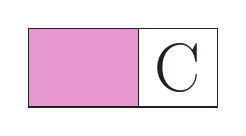
\begin{tikzpicture}[base]
    \widefont \Huge
        \draw [black, fill=C] (0,0) rectangle (1 + 0.4,1);
        \draw [black, fill=white] (1 + 0.4,0) rectangle (2 + 0.4,1);
        \node [,black] at (1.5 + 0.4,0.5) {\textbf C};
        \path [use as bounding box] (0,0) rectangle (2 + 0.4,1);
    \end{tikzpicture}
}

\newsavebox{\G}
\savebox{\G}{%
    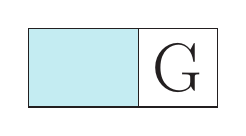
\begin{tikzpicture}[base]
    \widefont \Huge
        \draw [black, fill=G] (0,0) rectangle (1 + 0.4,1);
        \draw [black, fill=white] (1 + 0.4,0) rectangle (2 + 0.4,1);
        \node [,black] at (1.5 + 0.4,0.5) {\textbf G};
        \path [use as bounding box] (0,0) rectangle (2 + 0.4,1);
    \end{tikzpicture}
}

\newsavebox{\R}
\savebox{\R}{%
    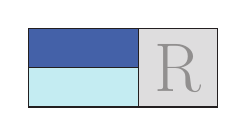
\begin{tikzpicture}[base]
    \widefont \Huge
        \draw [black, fill=G] (0,0) rectangle (1 + 0.4, 0.5);
        \draw [black, fill=A] (0,0.5) rectangle (1 + 0.4, 1);
        \draw [black, fill=lightgrey] (1 + 0.4,0) rectangle (2 + 0.4, 1);
        \node [,darkgrey] at (1.5 + 0.4,0.5) {\textbf R};
        \path [use as bounding box] (0,0) rectangle (2 + 0.4,1);
    \end{tikzpicture}
}

\newsavebox{\Y}
\savebox{\Y}{%
    
\begin{tikzpicture}[base]
    \widefont \Huge
        \draw [black, fill=C] (0,0) rectangle (1 + 0.4, 0.5);
        \draw [black, fill=U] (0,0.5) rectangle (1 + 0.4, 1);
        \draw [black, fill=lightgrey] (1 + 0.4,0) rectangle (2 + 0.4, 1);
        \node [,darkgrey] at (1.5 + 0.4,0.5) {\textbf Y};
        \path [use as bounding box] (0,0) rectangle (2 + 0.4,1);
    \end{tikzpicture}
}

\newsavebox{\HH}
\savebox{\HH}{%
    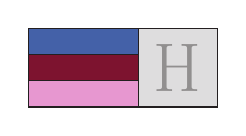
\begin{tikzpicture}[base]
    \widefont \Huge
        \draw [black, fill=C] (0,0) rectangle (1 + 0.4, 0.3333);
        \draw [black, fill=U] (0,0.3333) rectangle (1 + 0.4, 0.6666);
        \draw [black, fill=A] (0,0.6666) rectangle (1 + 0.4, 1);
        \draw [black, fill=lightgrey] (1 + 0.4,0) rectangle (2 + 0.4, 1);
        \node [,darkgrey] at (1.5 + 0.4,0.5) {\textbf H};
        \path [use as bounding box] (0,0) rectangle (2 + 0.4,1);
    \end{tikzpicture}
}

\newsavebox{\B}
\savebox{\B}{%
    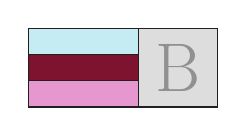
\begin{tikzpicture}[base]
    \widefont \Huge
        \draw [black, fill=C] (0,0) rectangle (1 + 0.4, 0.3333);
        \draw [black, fill=U] (0,0.3333) rectangle (1 + 0.4, 0.6666);
        \draw [black, fill=G] (0,0.6666) rectangle (1 + 0.4, 1);
        \draw [black, fill=lightgrey] (1 + 0.4,0) rectangle (2 + 0.4, 1);
        \node [,darkgrey] at (1.5 + 0.4,0.5) {\textbf B};
        \path [use as bounding box] (0,0) rectangle (2 + 0.4,1);
    \end{tikzpicture}
}

\newsavebox{\V}
\savebox{\V}{%
    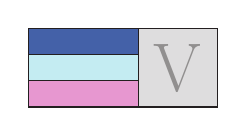
\begin{tikzpicture}[base]
    \widefont \Huge
        \draw [black, fill=C] (0,0) rectangle (1 + 0.4, 0.3333);
        \draw [black, fill=G] (0,0.3333) rectangle (1 + 0.4, 0.6666);
        \draw [black, fill=A] (0,0.6666) rectangle (1 + 0.4, 1);
        \draw [black, fill=lightgrey] (1 + 0.4,0) rectangle (2 + 0.4, 1);
        \node [,darkgrey] at (1.5 + 0.4,0.5) {\textbf V};
        \path [use as bounding box] (0,0) rectangle (2 + 0.4,1);
    \end{tikzpicture}
}

\newsavebox{\D}
\savebox{\D}{
    
\begin{tikzpicture}[base]
    \widefont \Huge
        \draw [black, fill=G] (0,0) rectangle (1 + 0.4, 0.3333);
        \draw [black, fill=U] (0,0.3333) rectangle (1 + 0.4, 0.6666);
        \draw [black, fill=A] (0,0.6666) rectangle (1 + 0.4, 1);
        \draw [black, fill=lightgrey] (1 + 0.4,0) rectangle (2 + 0.4, 1);
        \node [,darkgrey] at (1.5 + 0.4,0.5) {\textbf D};
        \path [use as bounding box] (0,0) rectangle (2 + 0.4,1);
    \end{tikzpicture}
}

\newsavebox{\W}
\savebox{\W}{%
    
\begin{tikzpicture}[base]
    \widefont \Huge
        \draw [black, fill=U] (0,0) rectangle (1 + 0.4, 0.5);
        \draw [black, fill=A] (0,0.5) rectangle (1 + 0.4, 1);
        \draw [black, fill=lightgrey] (1 + 0.4,0) rectangle (2 + 0.4, 1);
        \node [,darkgrey] at (1.5 + 0.4,0.5) {\textbf W};
        \path [use as bounding box] (0,0) rectangle (2 + 0.4,1);
    \end{tikzpicture}
}

\newsavebox{\SSS}
\savebox{\SSS}{%
    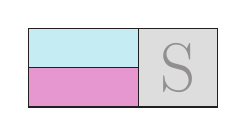
\begin{tikzpicture}[base]
    \widefont \Huge
        \draw [black, fill=C] (0,0) rectangle (1 + 0.4, 0.5);
        \draw [black, fill=G] (0,0.5) rectangle (1 + 0.4, 1);
        \draw [black, fill=lightgrey] (1 + 0.4,0) rectangle (2 + 0.4, 1);
        \node [,darkgrey] at (1.5 + 0.4,0.5) {\textbf S};
        \path [use as bounding box] (0,0) rectangle (2 + 0.4,1);
    \end{tikzpicture}
}

\newsavebox{\N}
\savebox{\N}{%
    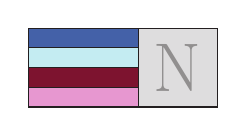
\begin{tikzpicture}[base]
    \widefont \Huge
        \draw [black, fill=C] (0,0) rectangle (1 + 0.4, 0.25);
        \draw [black, fill=U] (0,0.25) rectangle (1 + 0.4, 0.5);
        \draw [black, fill=G] (0,0.5) rectangle (1 + 0.4, 0.75);
        \draw [black, fill=A] (0,0.75) rectangle (1 + 0.4, 1);
        \draw [black, fill=lightgrey] (1 + 0.4,0) rectangle (2 + 0.4, 1);
        \node [,darkgrey] at (1.5 + 0.4,0.5) {\textbf N};
        \path [use as bounding box] (0,0) rectangle (2 + 0.4,1);
    \end{tikzpicture}
}


% greyed out versions for the delete action card

\newsavebox{\Agrey}
\savebox{\Agrey}{%
    
\begin{tikzpicture}[base]
    \widefont \Huge
        \draw [black, fill=darkgrey] (0,0) rectangle (1,1);
        \draw [black, fill=black] (1,0) rectangle (2,1);
        \node [,white] at (1.5,0.5) {\textbf A};
        \path [use as bounding box] (0,0) rectangle (2,1);
    \end{tikzpicture}
}

\newsavebox{\Tgrey}
\savebox{\Tgrey}{%
    
\begin{tikzpicture}[base]
    \widefont \Huge
        \draw [black, fill=darkgrey] (0,0) rectangle (1,1);
        \draw [black, fill=black] (1,0) rectangle (2,1);
        \node [,white] at (1.5,0.5) {\textbf T};
        \path [use as bounding box] (0,0) rectangle (2,1);
    \end{tikzpicture}
}

\newsavebox{\Cgrey}
\savebox{\Cgrey}{%
    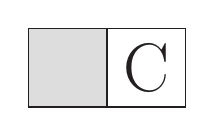
\begin{tikzpicture}[base]
    \widefont \Huge
        \draw [black, fill=lightgrey] (0,0) rectangle (1,1);
        \draw [black, fill=white] (1,0) rectangle (2,1);
        \node [,black] at (1.5,0.5) {\textbf C};
        \path [use as bounding box] (0,0) rectangle (2,1);
    \end{tikzpicture}
}

\newsavebox{\Ggrey}
\savebox{\Ggrey}{%
    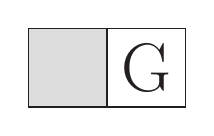
\begin{tikzpicture}[base]
    \widefont \Huge
        \draw [black, fill=lightgrey] (0,0) rectangle (1,1);
        \draw [black, fill=white] (1,0) rectangle (2,1);
        \node [,black] at (1.5,0.5) {\textbf G};
        \path [use as bounding box] (0,0) rectangle (2,1);
    \end{tikzpicture}
}


% larger versions for bleed in the corner on nt cards
% 0.4cm trims; TODOv2 make this dynamic

\newsavebox{\Acorner}
\savebox{\Acorner}{%
    
\begin{tikzpicture}[base]
    \widefont \Huge
        \draw [black, fill=A] (0,0) rectangle (1 + 0.4 ,1 + 0.4);
        \draw [black, fill=black] (1 + 0.4,0) rectangle (2 + 0.4,1 + 0.4);
        \node [,white] at (1.5 + 0.4 ,0.5) {\textbf A};
        \path [use as bounding box] (0,0) rectangle (2 + 0.4,1 + 0.4);
    \end{tikzpicture}
}

\newsavebox{\Tcorner}
\savebox{\Tcorner}{%
    
\begin{tikzpicture}[base]
    \widefont \Huge
        \draw [black, fill=T] (0,0) rectangle (1 + 0.4,1 + 0.4);
        \draw [black, fill=black] (1 + 0.4,0) rectangle (2 + 0.4,1 + 0.4);
        \node [,white] at (1.5 + 0.4,0.5) {\textbf T};
        \path [use as bounding box] (0,0) rectangle (2 + 0.4,1 + 0.4);
    \end{tikzpicture}
}

\newsavebox{\Ccorner}
\savebox{\Ccorner}{%
    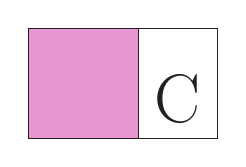
\begin{tikzpicture}[base]
    \widefont \Huge
        \draw [black, fill=C] (0,0) rectangle (1 + 0.4,1 + 0.4);
        \draw [black, fill=white] (1 + 0.4,0) rectangle (2 + 0.4,1 + 0.4);
        \node [,black] at (1.5 + 0.4,0.5) {\textbf C};
        \path [use as bounding box] (0,0) rectangle (2 + 0.4,1 + 0.4);
    \end{tikzpicture}
}

\newsavebox{\Gcorner}
\savebox{\Gcorner}{%
    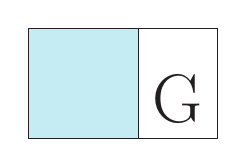
\begin{tikzpicture}[base]
    \widefont \Huge
        \draw [black, fill=G] (0,0) rectangle (1 + 0.4,1 + 0.4);
        \draw [black, fill=white] (1 + 0.4,0) rectangle (2 + 0.4,1 + 0.4);
        \node [,black] at (1.5 + 0.4,0.5) {\textbf G};
        \path [use as bounding box] (0,0) rectangle (2 + 0.4,1 + 0.4);
    \end{tikzpicture}
}


% no bleed versions for ac, instructions

\newsavebox{\Anb}
\savebox{\Anb}{%
    
\begin{tikzpicture}[base]
    \widefont \Huge
        \draw [black, fill=A] (0,0) rectangle (1,1);
        \draw [black, fill=black] (1,0) rectangle (2,1);
        \node [,white] at (1.5,0.5) {\textbf A};
        \path [use as bounding box] (0,0) rectangle (2,1);
    \end{tikzpicture}
}

\newsavebox{\Tnb}
\savebox{\Tnb}{%
    
\begin{tikzpicture}[base]
    \widefont \Huge
        \draw [black, fill=T] (0,0) rectangle (1,1);
        \draw [black, fill=black] (1,0) rectangle (2,1);
        \node [,white] at (1.5,0.5) {\textbf T};
        \path [use as bounding box] (0,0) rectangle (2,1);
    \end{tikzpicture}
}

\newsavebox{\Unb}
\savebox{\Unb}{%
    
\begin{tikzpicture}[base]
    \widefont \Huge
        \draw [black, fill=U] (0,0) rectangle (1,1);
        \draw [black, fill=black] (1,0) rectangle (2,1);
        \node [,white] at (1.5,0.5) {\textbf U};
        \path [use as bounding box] (0,0) rectangle (2,1);
    \end{tikzpicture}
}

\newsavebox{\Cnb}
\savebox{\Cnb}{%
    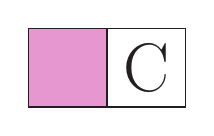
\begin{tikzpicture}[base]
    \widefont \Huge
        \draw [black, fill=C] (0,0) rectangle (1,1);
        \draw [black, fill=white] (1,0) rectangle (2,1);
        \node [,black] at (1.5,0.5) {\textbf C};
        \path [use as bounding box] (0,0) rectangle (2,1);
    \end{tikzpicture}
}

\newsavebox{\Gnb}
\savebox{\Gnb}{%
    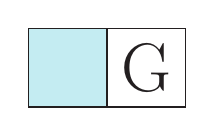
\begin{tikzpicture}[base]
    \widefont \Huge
        \draw [black, fill=G] (0,0) rectangle (1,1);
        \draw [black, fill=white] (1,0) rectangle (2,1);
        \node [,black] at (1.5,0.5) {\textbf G};
        \path [use as bounding box] (0,0) rectangle (2,1);
    \end{tikzpicture}
}

\newsavebox{\Rnb}
\savebox{\Rnb}{%
    
\begin{tikzpicture}[base]
    \widefont \Huge
        \draw [black, fill=G] (0,0) rectangle (1, 0.5);
        \draw [black, fill=A] (0,0.5) rectangle (1, 1);
        \draw [black, fill=lightgrey] (1,0) rectangle (2, 1);
        \node [,darkgrey] at (1.5,0.5) {\textbf R};
        \path [use as bounding box] (0,0) rectangle (2,1);
    \end{tikzpicture}
}

\newsavebox{\Ynb}
\savebox{\Ynb}{%
    
\begin{tikzpicture}[base]
    \widefont \Huge
        \draw [black, fill=C] (0,0) rectangle (1, 0.5);
        \draw [black, fill=U] (0,0.5) rectangle (1, 1);
        \draw [black, fill=lightgrey] (1,0) rectangle (2, 1);
        \node [,darkgrey] at (1.5,0.5) {\textbf Y};
        \path [use as bounding box] (0,0) rectangle (2,1);
    \end{tikzpicture}
}

\newsavebox{\HHnb}
\savebox{\HHnb}{%
    
\begin{tikzpicture}[base]
    \widefont \Huge
        \draw [black, fill=C] (0,0) rectangle (1, 0.3333);
        \draw [black, fill=U] (0,0.3333) rectangle (1, 0.6666);
        \draw [black, fill=A] (0,0.6666) rectangle (1, 1);
        \draw [black, fill=lightgrey] (1,0) rectangle (2, 1);
        \node [,darkgrey] at (1.5,0.5) {\textbf H};
        \path [use as bounding box] (0,0) rectangle (2,1);
    \end{tikzpicture}
}

\newsavebox{\Bnb}
\savebox{\Bnb}{%
    
\begin{tikzpicture}[base]
    \widefont \Huge
        \draw [black, fill=C] (0,0) rectangle (1, 0.3333);
        \draw [black, fill=U] (0,0.3333) rectangle (1, 0.6666);
        \draw [black, fill=G] (0,0.6666) rectangle (1, 1);
        \draw [black, fill=lightgrey] (1,0) rectangle (2, 1);
        \node [,darkgrey] at (1.5,0.5) {\textbf B};
        \path [use as bounding box] (0,0) rectangle (2,1);
    \end{tikzpicture}
}

\newsavebox{\Vnb}
\savebox{\Vnb}{%
    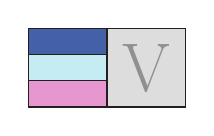
\begin{tikzpicture}[base]
    \widefont \Huge
        \draw [black, fill=C] (0,0) rectangle (1, 0.3333);
        \draw [black, fill=G] (0,0.3333) rectangle (1, 0.6666);
        \draw [black, fill=A] (0,0.6666) rectangle (1, 1);
        \draw [black, fill=lightgrey] (1,0) rectangle (2, 1);
        \node [,darkgrey] at (1.5,0.5) {\textbf V};
        \path [use as bounding box] (0,0) rectangle (2,1);
    \end{tikzpicture}
}

\newsavebox{\Dnb}
\savebox{\Dnb}{%
    
\begin{tikzpicture}[base]
    \widefont \Huge
        \draw [black, fill=G] (0,0) rectangle (1, 0.3333);
        \draw [black, fill=U] (0,0.3333) rectangle (1, 0.6666);
        \draw [black, fill=A] (0,0.6666) rectangle (1, 1);
        \draw [black, fill=lightgrey] (1,0) rectangle (2, 1);
        \node [,darkgrey] at (1.5,0.5) {\textbf D};
        \path [use as bounding box] (0,0) rectangle (2,1);
    \end{tikzpicture}
}

\newsavebox{\Wnb}
\savebox{\Wnb}{%
    
\begin{tikzpicture}[base]
    \widefont \Huge
        \draw [black, fill=U] (0,0) rectangle (1, 0.5);
        \draw [black, fill=A] (0,0.5) rectangle (1, 1);
        \draw [black, fill=lightgrey] (1,0) rectangle (2, 1);
        \node [,darkgrey] at (1.5,0.5) {\textbf W};
        \path [use as bounding box] (0,0) rectangle (2,1);
    \end{tikzpicture}
}

\newsavebox{\SSSnb}
\savebox{\SSSnb}{%
    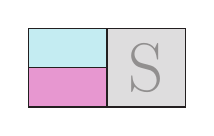
\begin{tikzpicture}[base]
    \widefont \Huge
        \draw [black, fill=C] (0,0) rectangle (1, 0.5);
        \draw [black, fill=G] (0,0.5) rectangle (1, 1);
        \draw [black, fill=lightgrey] (1,0) rectangle (2, 1);
        \node [,darkgrey] at (1.5,0.5) {\textbf S};
        \path [use as bounding box] (0,0) rectangle (2,1);
    \end{tikzpicture}
}

\newsavebox{\Knb}
\savebox{\Knb}{%
    
\begin{tikzpicture}[base]
    \widefont \Huge
        \draw [black, fill=T] (0,0) rectangle (1, 0.5);
        \draw [black, fill=G] (0,0.5) rectangle (1, 1);
        \draw [black, fill=lightgrey] (1,0) rectangle (2, 1);
        \node [,darkgrey] at (1.5,0.5) {\textbf K};
        \path [use as bounding box] (0,0) rectangle (2,1);
    \end{tikzpicture}
}

\newsavebox{\Mnb}
\savebox{\Mnb}{%
    
\begin{tikzpicture}[base]
    \widefont \Huge
        \draw [black, fill=A] (0,0) rectangle (1, 0.5);
        \draw [black, fill=C] (0,0.5) rectangle (1, 1);
        \draw [black, fill=lightgrey] (1,0) rectangle (2, 1);
        \node [,darkgrey] at (1.5,0.5) {\textbf M};
        \path [use as bounding box] (0,0) rectangle (2,1);
    \end{tikzpicture}
}

\newsavebox{\Nnb}
\savebox{\Nnb}{%
    
\begin{tikzpicture}[base]
    \widefont \Huge
        \draw [black, fill=C] (0,0) rectangle (1, 0.25);
        \draw [black, fill=U] (0,0.25) rectangle (1, 0.5);
        \draw [black, fill=G] (0,0.5) rectangle (1, 0.75);
        \draw [black, fill=A] (0,0.75) rectangle (1, 1);
        \draw [black, fill=lightgrey] (1,0) rectangle (2, 1);
        \node [,darkgrey] at (1.5,0.5) {\textbf N};
        \path [use as bounding box] (0,0) rectangle (2,1);
    \end{tikzpicture}
}


%%%%%%%%%%%%%%%%%%%%%%%%%%%%%%%%%%%%%%%%%%%%%%%%%%%%%%%%%%%%%%%%%%%%%%%%%%%%%%%%
%  Draw the molecules
%%%%%%%%%%%%%%%%%%%%%%%%%%%%%%%%%%%%%%%%%%%%%%%%%%%%%%%%%%%%%%%%%%%%%%%%%%%%%%%%

\usepackage{chemfig}
\renewcommand*\printatom[1]{\ensuremath{\mathsf{#1}}}
\setnodestyle{inner sep=0pt, outer sep=0pt, scale=0.9}
\setbondstyle{cap=round, line width=2pt}
\setdoublesep{5pt}
\setatomsep{25pt}
\setbondoffset{3pt}

\tikzset{
  hbond/.style={dotted,blue}
}

\definesubmol{amino}{ {\textcolor{gray}{H_2}}|{\textcolor{gray} N}-[:-30,,,,gray,] }
\definesubmol{acid}{ -[:30,,,,gray,](=[:90,,,,gray,]{\textcolor{gray}{O}})-[:-30,,,,gray,]{\textcolor{gray}O}|{\textcolor{gray}H} }

\newcommand{\molecule}[1]{
    \LARGE #1
}

% amino acids

\newcommand{\alanine}{
    \chemfig[][scale=1.1]{!{amino}(-[:270])!{acid}}
}
\newcommand{\arginine}{
    \chemfig[][scale=1.05]{!{amino}(-[:270]-[:210]-[:270]-[:210]N=[:270](-[:330]NH_2)(-[:210]H_2N))!{acid}}
}
\newcommand{\asparagine}{
    \chemfig[][scale=1.1]{!{amino}(-[:270]-[:210](-[:270]NH_2)(=[:150]O))!{acid}}
}
\newcommand{\aspartate}{
    \chemfig[][scale=1.1]{!{amino}(-[:270]-[:210](-[:270]OH)(=[:150]O))!{acid}}
}
\newcommand{\cysteine}{
    \chemfig[][scale=1.1]{!{amino}(-[:270]-[:210]HS)!{acid}}
}
\newcommand{\glutamine}{
    \chemfig[][scale=1.1]{!{amino}(-[:270]-[:210]-[:270](=[:330]O)(-[:210]H_2N))!{acid}}
}
\newcommand{\glutamate}{
    \chemfig[][scale=1.1]{!{amino}(-[:270]-[:210]-[:270](=[:330]O)(-[:210]HO))!{acid}}
}
\newcommand{\glycine}{
    \chemfig[][scale=1.1]{!{amino}()!{acid}}
}
\newcommand{\histidine}{
    \chemfig[][scale=1.1]{!{amino}(-[:270]-[:210]*5(=-N=-[,,1,1]NH-[,,1,1]))!{acid}}
}
\newcommand{\isoleucine}{
    \chemfig[][scale=1.1]{!{amino}(-[:270](-[:210]-[:270])(-[:330]))!{acid}}
}
\newcommand{\leucine}{
    \chemfig[][scale=1.1]{!{amino}(-[:270]-[:210](-[:270])(-[:150]))!{acid}}
}
\newcommand{\lysine}{
    \chemfig[][scale=1.1]{!{amino}(-[:270]-[:210]-[:270]-[:210]-[:270]NH_2)!{acid}}
}
\newcommand{\methionine}{
    \chemfig[][scale=1.1]{!{amino}(-[:270]-[:210]-[:270]S-[:210])!{acid}}
}
\newcommand{\phenylalanine}{
    \chemfig[line width=2pt, scale=1.1][scale=1.1]{!{amino}(-[:270]-[:210]**6(------))!{acid}}
}
\newcommand{\proline}{
    \chemfig[][scale=1.1]{([:30](=[:90,,,,gray,]{\textcolor{gray}{O}})(-[:330,,,,gray,]{\textcolor{gray}{O}}|{\textcolor{gray}{H}}))(-[:210,,,,gray,]*5(-[,,,2,gray,]{\textcolor{gray}{H}}|{\textcolor{gray}{N}}-[,,2,]---))}
}
\newcommand{\serine}{
    \chemfig[][scale=1.1]{!{amino}(-[:270]-[:210]HO)!{acid}}
}
\newcommand{\threonine}{
    \chemfig[][scale=1.1]{!{amino}(-[:270](-[:210]HO)(-[:330]))!{acid}}
}
\newcommand{\tryptophan}{
    \chemfig[line width=2pt, scale=1.1][scale=1.1]{!{amino}(-[:270]-[:210]*5(=-HN-**6(------)--))!{acid}}
}
\newcommand{\tyrosine}{
    \chemfig[line width=2pt, scale=1.1][scale=1.1]{!{amino}(-[:270]-[:210]**6(---(-HO)---))!{acid}}
}
\newcommand{\valine}{
    \chemfig[][scale=1.1]{!{amino}(-[:270](-[:210])(-[:330]))!{acid}}
}


% bases

\newcommand{\adenine}{
    %\chemfig[line width=2pt, scale=1.1][scale=1.1]{[:-120]-[,2]*5(-[,,,2]HN-[,,2,]*6(-N=-@{a2}N=(-@{a1}NH_2)-=)--N=-)}  % doesn't work -[,,,2]HN-[,,2,]
    \chemfig[line width=2pt, scale=1.1][scale=1.1]{[:-210]N@{a1}H_2-*6(-*5(-N=(-[,2])-[,,,2]HN-[,,2]-)=-N=-@{a2}N=)}     % exactly the same but works
}

\newcommand{\thymine}{
    %\chemfig[line width=2pt, scale=1.1][scale=1.1]{[:60]-[,2]N*6(-=(-CH_3)-(=@{t1}O)-[,,,2]@{t2}HN-[,,2,](=O)-)}
    \chemfig[line width=2pt, scale=1.1, rotate=180][scale=1.1, rotate=180]{[:-120]-[,2]N*6(-=(-H_3C)-(=@{t1}O)-[,,,1]N@{t2}H-[,,1,](=O)-)}
    %@{t2}HN*6(-(=O)-N(-)-=(-CH_3)-(=@{t1}O)-)}
}


\newcommand{\hbondat}{
    \chemmove{ \draw[lightgray, line width=4pt, line cap=round, shorten >= 10pt, shorten <= 5pt, dash pattern = on 0.5pt off 8pt] (a1) to[out=270,in=50] (t1); }
    \chemmove{ \draw[lightgray, line width=4pt, line cap=round, shorten >=10pt, shorten <=5pt, dash pattern = on 0.5pt off 8pt] (a2) to[out=230,in=115] (t2); }
}

\newcommand{\guanine}{
    %\chemfig[line width=2pt, scale=1.1][scale=1.1]{[:120]-[,2]N*5(-*6(-N=(-@{g3}NH_2)-[,,,1]@{g2}NH-[,,1,](=@{g1}O)-=)--N=-)}
    \chemfig[line width=2pt, scale=1.1, rotate=180][scale=1.1, rotate=180]{[:-60]-[,2]N*5(-*6(-N=(-@{g3}H_2N)-[,,,2]@{g2}HN-[,,2,](=@{g1}O)-=)--N=-)}
}

\newcommand{\cytosine}{
    \chemfig[line width=2pt, scale=1.1][scale=1.1]{[:-120]-[,2]N*6(-=-(-@{c1}H_2N)=@{c2}N-(=@{c3}O)-)}
}

\newcommand{\hbondgc}{
    \chemmove{ \draw[lightgray, line width=4pt, line cap=round, shorten >=3pt, shorten <=17pt, dash pattern = on 0.5pt off 8pt] (g1) to[out=110, in=250] (c1); }
    \chemmove{ \draw[lightgray, line width=4pt, line cap=round, shorten >=5pt, shorten <=17pt, dash pattern = on 0.5pt off 8pt] (g2) to[out=65, in=300] (c2); }
    \chemmove{ \draw[lightgray, line width=4pt, line cap=round, shorten >=2pt, shorten <=17pt, dash pattern = on 0.5pt off 8pt] (g3) to[out=45, in=320] (c3); }
}


%%%%%%%%%%%%%%%%%%%%%%%%%%%%%%%%%%%%%%%%%%%%%%%%%%%%%%%%%%%%%%%%%%%%%%%%%%%%%%%%%%%
%  Macros for the Amino acid cards
%%%%%%%%%%%%%%%%%%%%%%%%%%%%%%%%%%%%%%%%%%%%%%%%%%%%%%%%%%%%%%%%%%%%%%%%%%%%%%%%

\usetikzlibrary{shapes}

\newcommand{\codon}[3]{%
        \node [anchor=west, yshift=2.5cm] at (stock page.west) {\usebox{#1}};
        \node [anchor=west, yshift=1.5cm] at (stock page.west) {\usebox{#2}};
        \node [anchor=west, yshift=0.5cm] at (stock page.west) {\usebox{#3}};
}

\newcommand{\codons}[6]{%
        \node [anchor=west, yshift=2.5cm] at (stock page.west) {\usebox{#1}};
        \node [anchor=west, yshift=1.5cm] at (stock page.west) {\usebox{#2}};
        \node [anchor=west, yshift=0.5cm] at (stock page.west) {\usebox{#3}};
        \node [anchor=west, yshift=-1cm] at (stock page.west) {\usebox{#4}};
        \node [anchor=west, yshift=-2cm] at (stock page.west) {\usebox{#5}};
        \node [anchor=west, yshift=-3cm] at (stock page.west) {\usebox{#6}};
}

\newcommand{\group}[2]{
    \narrowfont
    \node (first) [anchor = west, xshift=-1cm, yshift=0.5cm] at (trimmed page.south east) {#1};
    \node (firsttext) [anchor=east, left=0.2 of first.west] {\scalefont{1.4}{#2}};
}
\newcommand{\groups}[4]{
    \narrowfont 
    \node (first) [anchor = west, xshift=-1cm, yshift=0.5cm] at (trimmed page.south east) {#1};
    \node (firsttext) [anchor=east, left=0.2 of first.west] {\scalefont{1.4}{#2}};
    \node (second) [anchor = west, xshift=-1cm, yshift=1.25cm] at (trimmed page.south east) {#3};
    \node (secondtext) [anchor=east, left = 0.2 of second.west] {\scalefont{1.4}{#4}};
}

\newcommand{\namealiphatic}{Aliphatic}
\newcommand{\namearomatic}{Aromatic}
\newcommand{\nameunusual}{Unusual}
\newcommand{\nameacidic}{Acidic}
\newcommand{\namebasic}{Basic}
\newcommand{\nameacidderiv}{Acid Deriv.}
\newcommand{\namesmallpolar}{Small Polar}
\newcommand{\namesulfur}{Sulfur}


% TODOv2 maybe merge this: use saveboxes for instructions and commands for cards

\newsavebox{\basicbox}
\savebox{\basicbox}{%
    
\begin{tikzpicture}[base, overlay]
        \draw (0,0) circle (0.17);
        \draw [line width=1pt] (-0.11, 0) -- (0.11,0);
        \draw [line width=1pt] (0, -0.11) -- (0, 0.11);
        \path[use as bounding box] (-0.17, -0.17) rectangle (0.17, 0.17);
    \end{tikzpicture}
}

\newcommand{\basic}{
	
\begin{tikzpicture}[base]
        \draw (0,0) circle (0.17);
        \draw [line width=1pt] (-0.11, 0) -- (0.11,0);
        \draw [line width=1pt] (0, -0.11) -- (0, 0.11);
        \path[use as bounding box] (-0.17, -0.17) rectangle (0.17, 0.17);
    \end{tikzpicture}
}

\newsavebox{\acidicbox}
\savebox{\acidicbox}{%
    
\begin{tikzpicture}[base, overlay]
        \draw (0,0) circle (0.17);
        \draw [line width=1pt] (-0.11, 0) -- (0.11,0);
        \path[use as bounding box] (-0.17, -0.17) rectangle (0.17, 0.17);
    \end{tikzpicture}
}

\newcommand{\acidic}{
	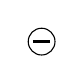
\begin{tikzpicture}[base]
        \draw (0,0) circle (0.17);
        \draw [line width=1pt] (-0.11, 0) -- (0.11,0);
        \path[use as bounding box] (-0.17, -0.17) rectangle (0.17, 0.17);
    \end{tikzpicture}
}


\newsavebox{\aromaticbox}
\savebox{\aromaticbox}{%
    \begin{tikzpicture}[base, overlay]
    \node at (0,0) { \chemfig[scale=0.2, line width=0.5pt][scale=0.2]{**6(-[,,,,,line width=1.0pt]-[,,,,,line width=1.0pt]-[,,,,,line width=1.0pt]-[,,,,,line width=1.0pt]-[,,,,,line width=1.0pt]-[,,,,,line width=1.0pt])}};
    \end{tikzpicture}
}

\newcommand{\aromatic}{
    \chemfig[scale=0.25, line width=0.5pt][scale=0.25]{**6(-[,,,,,line width=1.0pt]-[,,,,,line width=1.0pt]-[,,,,,line width=1.0pt]-[,,,,,line width=1.0pt]-[,,,,,line width=1.0pt]-[,,,,,line width=1.0pt])}
}


\newsavebox{\aliphaticbox}
\savebox{\aliphaticbox}{%
    \begin{tikzpicture}[base, overlay]
    \node at (0,0) { \chemfig[][scale=0.3]{-[:30,,,,,line width=1.0pt]-[:-30,,,,,line width=1.0pt]-[:30,,,,,line width=1.0pt]} };
    \end{tikzpicture}
}

\newcommand{\aliphatic}{
    %\chemfig[][scale=0.3]{-[:30,,,,,line width=1pt]-[:-30,,,,,line width=1pt]-[:30,,,,,line width=1pt]-[:-30,,,,,line width=1pt]-[:30,,,,,line width=1pt]}
    \chemfig[][scale=0.3]{-[:30,,,,,line width=1.0pt]-[:-30,,,,,line width=1.0pt]-[:30,,,,,line width=1.0pt]}
}


\newsavebox{\sulfurbox}
\savebox{\sulfurbox}{%
    
\begin{tikzpicture}[base, overlay]
        \narrowfont
        \scalefont{.8}{} \selectfont
        \node [draw, regular polygon,regular polygon sides=6, minimum size=.3] at (0,0) {S};
    \end{tikzpicture}
}

\newcommand{\sulfur}{
	
\begin{tikzpicture}[base]
        \node [draw, regular polygon,regular polygon sides=6, minimum size=.3] at (0,0) {S};
        %\path[use as bounding box] (-0.15, -0.15) rectangle (0.15, 0.15);
    \end{tikzpicture}
}


\newsavebox{\acidderivbox}
\savebox{\acidderivbox}{%
    
\begin{tikzpicture}[base, overlay]
        \narrowfont
        \scalefont{.8}{} \selectfont
        \node [draw, regular polygon,regular polygon sides=7, minimum size=.3] at (0,0) {N};
    \end{tikzpicture}
}

\newcommand{\acidderiv}{
	
\begin{tikzpicture}[base]
        \node [draw, regular polygon,regular polygon sides=7, minimum size=.3] at (0,0) {N};
        %\path[use as bounding box] (-0.15, -0.15) rectangle (0.15, 0.15);
    \end{tikzpicture}
}


\newsavebox{\smallpolarbox}
\savebox{\smallpolarbox}{%
    
\begin{tikzpicture}[base, overlay]
        \draw [line width=1pt] (-0.15,-0.15) -- (0.15,-0.15) arc (-90:90:0.15) -- (-0.15,0.15) arc (90:270:0.15);
        \draw (-0.24, 0) -- (-0.06,0);
        \draw (-0.15, -0.09) -- (-0.15, 0.09);
        \draw (0.06, 0) -- (0.24,0);
    \end{tikzpicture}
}

\newcommand{\smallpolar}{
	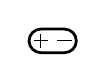
\begin{tikzpicture}[base]
        \draw [line width=1pt] (0,-0.15) -- (0.30,-0.15) arc (-90:90:0.15) -- (0,0.15) arc (90:270:0.15);
        \draw (-0.09, 0) -- (0.09,0);
        \draw (0, -0.09) -- (0, 0.09);
        \draw (0.21, 0) -- (0.39,0);
        %\path[use as bounding box] (-0.15, -0.15) rectangle (0.6, 0.15);
    \end{tikzpicture}
}

\newsavebox{\unusualbox}
\savebox{\unusualbox}{%
    \begin{tikzpicture}[base, overlay]
        \draw (0,0) circle (0.15);
        \draw (0,0) circle (0.05);
        \draw (0,0.1) circle (0.05);
        \draw (0.1,0) circle (0.05);
        \draw (-0.1,0) circle (0.05);
        \draw (0,-0.1) circle (0.05);
        \draw (-0.18, 0) -- (0.18,0);
        \draw (0, -0.18) -- (0, 0.18);
        \path[use as bounding box] (-0.17, -0.17) rectangle (0.17, 0.17);
    \end{tikzpicture}
}



\newcommand{\unusual}{
	\begin{tikzpicture}[base]
        \draw (0,0) circle (0.15);
        \draw (0,0) circle (0.05);
        \draw (0,0.1) circle (0.05);
        \draw (0.1,0) circle (0.05);
        \draw (-0.1,0) circle (0.05);
        \draw (0,-0.1) circle (0.05);
        \draw (-0.18, 0) -- (0.18,0);
        \draw (0, -0.18) -- (0, 0.18);
        \path[use as bounding box] (-0.17, -0.17) rectangle (0.17, 0.17);
    \end{tikzpicture}
}

\newsavebox{\hydro}
\savebox{\hydro}{%
    \begin{tikzpicture}[base]
        % counterclockwise: bottom, farthest right, top point, farthest left, bottom
        \draw [fill=lightblue] (0,0) to[out=0,in=-90] (0.18,0.21) to[out=90,in=250] (0.014,0.6) to [out=215, in=90] (-0.225,0.225) to [out=270, in=180] (0,0);
        \path[use as bounding box] (-0.15, 0) rectangle (0.12, 0.4);
    \end{tikzpicture}
}

\newsavebox{\hydrotiny}
\savebox{\hydrotiny}{%
    \begin{tikzpicture}[base, overlay]
        % counterclockwise: bottom, farthest right, top point, farthest left, bottom
        %\draw [fill=lightblue] (0,0) to[out=0,in=-90] (0.12,0.14) to[out=90,in=250] (0.01,0.4) to [out=215, in=90] (-0.15,0.15) to [out=270, in=180] (0,0);
        %\draw [fill=lightblue] (0,0) to[out=0,in=-90] (0.06,0.07) to[out=90,in=250] (0.005,0.2) to [out=215, in=90] (-0.075,0.0715) to [out=270, in=180] (0,0);
        \draw [fill=lightblue] (0,0) to[out=0,in=-90] (0.09,0.105) to[out=90,in=250] (0.0075,0.3) to [out=215, in=90] (-0.1125,0.1125) to [out=270, in=180] (0,0);
        \path[use as bounding box] (0, 0) rectangle (-0.1, 0.1);
    \end{tikzpicture}
}

\newsavebox{\hydrobig}
\savebox{\hydrobig}{%
    \begin{tikzpicture}[base]
        % counterclockwise: bottom, farthest right, top point, farthest left, bottom
        \draw [thick, fill=lightblue] (0,0) to[out=0,in=-90] (0.48,0.56) to[out=90,in=250] (0.04,1.6) to [out=215, in=90] (-0.6,0.6) to [out=270, in=180] (0,0);
        \path[use as bounding box] (-0.6, 0) rectangle (0.48, 1.6);
    \end{tikzpicture}
}

\newsavebox{\hydrobigwhite}
\savebox{\hydrobigwhite}{%
    \begin{tikzpicture}[base]
        % counterclockwise: bottom, farthest right, top point, farthest left, bottom
        \draw [thick, fill=white] (0,0) to[out=0,in=-90] (0.48,0.56) to[out=90,in=250] (0.04,1.6) to [out=215, in=90] (-0.6,0.6) to [out=270, in=180] (0,0);
        \path[use as bounding box] (-0.6, 0) rectangle (0.48, 1.6);
    \end{tikzpicture}
}

%%%%%%%%%%%%%%%%%%%%%%%%%%%%%%%%%%%%%%%%%%%%%%%%%%%%%%%%%%%%%%%%%%%%%%%%%%%%%
%  Amino acid card
%%%%%%%%%%%%%%%%%%%%%%%%%%%%%%%%%%%%%%%%%%%%%%%%%%%%%%%%%%%%%%%%%%%%%%%%%%%%%%%%
\usetikzlibrary{matrix}



\newcommand{\aacard}[7]{
    \begin{tikzpicture}[card]
       
        % one letter code
        \node[anchor = north west, xshift=0.125cm, yshift=-0.25cm](letter) at (trimmed page.north west) { \widefont\Huge\textcolor{black}{\textbf{\scalefont{2}#1\\}} };

        % three letter code
        \node[right = 0.1cm of letter.north east, anchor = north west, baseline] (threeletter) { \textcolor{black}{#2\\} };

        \ifthenelse{\equal{#7}{hydrophilic}}
           { 
                \node[anchor=south west, right=0.1cm of letter.south east, yshift=0.3cm] {\usebox{\hydro}};
           }
           {}


        % name
        \node[anchor = north east, xshift=-0.25cm, yshift=-0.25cm] (name) at (trimmed page.north east) { \narrowfont\Huge\sffamily \textbf{#3} };


        % codon(s)
        #4;

        % molecule
        \ifthenelse{\equal{#1}{Y}}
        {
            \node[xshift = 0.3cm] at (trimmed page.center) {#5};
        }
        {
            \node[xshift = 1cm] at (trimmed page.center) {#5};
        }

        % group(s) 
        #6;

    \end{tikzpicture}
    \clearpage
}


\newcommand{\sq}[1]{
\draw[fill=#1, draw=none] (0,0) rectangle (\textwidth * 0.083333, \textheight * 0.0625); 
}

\newcommand{\sqt}[1]{
\draw[fill=#1, draw=none] (0,0) rectangle (\textwidth * 0.083333, \textheight * 0.0625 + \trimtop); 
}

\newcommand{\sqe}[1]{
\draw[fill=#1, draw=none] (0,0) rectangle (\textwidth * 0.083333 + \trimedge, \textheight * 0.0625); 
}

\newcommand{\sqc}[1]{
\draw[fill=#1, draw=none] (0,0) rectangle (\textwidth * 0.083333 + \trimedge, \textheight * 0.0625 + \trimtop); 
}

\newcommand{\sqq}[1]{
\draw[fill=#1, draw=none] (0,0) rectangle (\textwidth * 0.5 + \trimedge, \textheight * 0.5 + \trimtop); 
}

\newcommand{\aaback} {
}


%%%%%%%%%%%%%%%%%%%%%%%%%%%%%%%%%%%%%%%%%%%%%%%%%%%%%%%%%%%%%%%%%%%%%%%%%%%%%%%%
%  Nucleotide card
%%%%%%%%%%%%%%%%%%%%%%%%%%%%%%%%%%%%%%%%%%%%%%%%%%%%%%%%%%%%%%%%%%%%%%%%%%%%%%%%

\newcommand{\ntcard}[2] {
    \begin{tikzpicture}[card]
        \node[anchor=north west] at (stock page.north west) {\usebox{#1}};
        \node[anchor=north west, rotate = 180] at (stock page.south east) {\usebox{#2}};

        \ifthenelse{\equal{#1}{\Acorner}}
        {
            \node[anchor=north] at (stock page.north) {\molecule{\adenine}};
            \node[anchor=south] at (stock page.south) {\molecule{\thymine}};
            \hbondat;
        }
        {
            \node[anchor=north] at (stock page.north) {\molecule{\cytosine}};
            \node[anchor=south] at (stock page.south) {\molecule{\guanine}};
            \hbondgc;
        }

    \end{tikzpicture}    
    \clearpage
}


%%%%%%%%%%%%%%%%%%%%%%%%%%%%%%%%%%%%%%%%%%%%%%%%%%%%%%%%%%%%%%%%%%%%%%%%%%%%%%%%
%  Game accessory cards
%%%%%%%%%%%%%%%%%%%%%%%%%%%%%%%%%%%%%%%%%%%%%%%%%%%%%%%%%%%%%%%%%%%%%%%%%%%%%%%%

\newcommand{\watercardon} {
}

\newcommand{\watercardoff} {
}

\newcommand{\fiveprime} {
    \begin{tikzpicture}[card]
        \node [yshift=-1cm,xshift=0.5cm](arrowtail) at (trimmed page.north west) [] { };
        \node [yshift=-1cm,xshift=-0.5cm](arrowhead) at (trimmed page.north east) [] { };
        \node[yshift=-0.5cm](five) at (trimmed page.center) {\fontsize{200}{200} \selectfont 5'};
        \draw[-latex, line width=12pt] (arrowtail) -- (arrowhead);

        %\node [yshift=0.5cm,xshift=-0.7cm](littletail) at (trimmed page.south east) [] { };
        %\node [yshift=0.51cm,xshift=-1.5cm](littlehead) at (trimmed page.south east) [] { };
        %\draw[-latex, line width=1pt, color=grey] (littletail) -- (littlehead);
        %\node[text=grey, rotate=180, xshift=1cm, yshift=-1cm] at (trimmed page.south east) {\fontsize{20}{20} \selectfont 3'};
    \end{tikzpicture}
    \clearpage
}

\newcommand{\threeprime} {
    \begin{tikzpicture}[card]
        \node [xshift=0cm,yshift=1cm,xshift=0.5cm](arrowtail) at (trimmed page.south west) [] { };
        \node [xshift=0cm,yshift=1cm,xshift=-0.5cm](arrowhead) at (trimmed page.south east) [] { };

        \node[yshift=0.5cm, text=grey, rotate=180](five) at (trimmed page.center) {\fontsize{200}{200} \selectfont 3'};
        \draw[latex-, line width=12pt, color=grey] (arrowtail) -- (arrowhead);

        \node [yshift=-0.5cm,xshift=0.7cm](littletail) at (trimmed page.north west) [] { };
        \node [yshift=-0.51cm,xshift=1.5cm](littlehead) at (trimmed page.north west) [] { };
        \draw[-latex, line width=1pt, color=black] (littletail) -- (littlehead);
        \node[text=black, xshift=1cm, yshift=-1cm] at (trimmed page.north west) {\fontsize{20}{20} \selectfont 5'};
    \end{tikzpicture}
    \clearpage
}

\newcommand{\referencent} {
    \begin{tikzpicture}[card]
        \node (C) [anchor=south, inner sep=2mm, label=below:{Cytosine}, yshift=-5mm] at (trimmed page.center) {\usebox{\Cnb}};
        \node (T) [inner sep=2mm, left= -0.1cm of C, label=below:{Thymine}] {\usebox{\Tnb}};
        \node (Y) [inner sep=2mm, right= -0.1cm of C, label=below:{Pyrimidine}] {\usebox{\Ynb}};

        \node (G) [inner sep=2mm, above= 0.5cm of C, label=below:{Guanine}] {\usebox{\Gnb}};
        \node (A) [inner sep=2mm, above= 0.5cm of T, label=below:{Adenine}] {\usebox{\Anb}};
        \node (R) [inner sep=2mm, above= 0.5cm of Y, label=below:{Purine}] {\usebox{\Rnb}};

        \node (S) [inner sep=2mm, above= 0.5cm of G, label=below:{Strong}] {\usebox{\SSSnb}};
        \node (W) [inner sep=2mm, above= 0.5cm of A, label=below:{Weak}] {\usebox{\Wnb}};
        \node (K) [inner sep=2mm, above= 0.5cm of R, label=below:{Keto}] {\usebox{\Knb}};

        \node (H) [inner sep=2mm, below= 0.5cm of C, label=below:{Not G}] {\usebox{\HHnb}};
        \node (B) [inner sep=2mm, below= 0.5cm of T, label=below:{Not A}] {\usebox{\Bnb}};
        \node (M) [inner sep=2mm, below= 0.5cm of Y, label=below:{Amino}] {\usebox{\Mnb}};

        \node (D) [inner sep=2mm, below= 0.5cm of H, label=below:{Not C}] {\usebox{\Dnb}};
        \node (V) [inner sep=2mm, below= 0.5cm of B, label=below:{Not T}] {\usebox{\Vnb}};
        \node (N) [inner sep=2mm, below= 0.5cm of M, label=below:{Any}] {\usebox{\Nnb}};

    \end{tikzpicture}    
    \clearpage
}

\newcommand{\referencemutation} {
    \begin{tikzpicture}[card]
        \node (G) [rotate=90, anchor=north east, xshift=-1.0cm, yshift=-0.5cm] at (trimmed page.north west) {\usebox{\Gnb}};
        \node (C) [rotate=90, anchor=south east, xshift=-1.0cm, yshift=0.5cm] at (trimmed page.north east) {\usebox{\Cnb}};
        \node (A) [rotate=90, anchor=north west, xshift=1.0cm, yshift=-0.5cm] at (trimmed page.south west) {\usebox{\Anb}};
        \node (T) [rotate=90, anchor=south west, xshift=1.0cm, yshift=0.5cm] at (trimmed page.south east) {\usebox{\Tnb}};

    \path
        (A) edge[mut, sloped] node {Transition}   (G)
            edge[mut] node {}             (C)
        (G) edge[mut] node {} (T)
        (T) edge[mut, sloped] node {Transition}   (C)
            edge[mut] node {}   (A)
        (C) edge[mut] node {}   (G)
        ;

        \node [rotate=90, anchor=center] at ($(A)!0.5!(T)$) {Complement};
        \node [rotate=90, anchor=center] at ($(G)!0.5!(C)$) {Complement};
        \node [rotate=90, anchor=center] at ($(T)!0.5!(G)$) {Transversion};

    \end{tikzpicture}    
    \clearpage
}


\newcommand{\referencegroups} {
    \begin{tikzpicture}[card]
        \node (AL) at (1,-1)     {\aliphatic{}};
        \node [below=of AL, node distance=0.5cm] (AR) {\aromatic{}};
        \node [below=of AR] (SP) {\smallpolar{}};
        \node [below=of SP] (BA) {\basic{}};
        \node [below=of BA] (AC) {\acidic{}};
        \node [below=of AC] (AD) {\acidderiv{}};
        \node [below=of AD] (SU) {\sulfur{}};
        \node [below=of SU] (UN) {\unusual{}};
    \end{tikzpicture}    
    \clearpage
}

\newcommand{\turnsummaryfront} {
    \begin{tikzpicture}[card]
        \node at (trimmed page.center) {placeholder turn summary front};
    \end{tikzpicture}    
    \clearpage
}

\newcommand{\turnsummaryback} {
    \begin{tikzpicture}[card]
        \node at (trimmed page.center) {placeholder turn summary back};
    \end{tikzpicture}    
    \clearpage
}


%%%%%%%%%%%%%%%%%%%%%%%%%%%%%%%%%%%%%%%%%%%%%%%%%%%%%%%%%%%%%%%%%%%%%%%%%%%%%
%  Action cards
%%%%%%%%%%%%%%%%%%%%%%%%%%%%%%%%%%%%%%%%%%%%%%%%%%%%%%%%%%%%%%%%%%%%%%%%%%%%%%%%

\newcommand{\acback} {
}


\newcommand{\togglewater} {
    \begin{tikzpicture}[card]
        \node[anchor = north west, xshift=0.25cm, yshift=-0.25cm] (action) at (trimmed page.north west) { \narrowfont\Huge\sffamily \textbf{Toggle Water ON/OFF}};
        \node[below = 3cm, text width=5cm] at (trimmed page.center) {Turn the water on or off. };

        \node (leftlevel)   [yshift=-5.0cm]               at (stock page.north west) {};
        \node (firstpeak)   [yshift=-4.6cm, xshift=4.0cm] at (stock page.north west) {};
        \node (firsttrough) [yshift=-4.8cm, xshift=5.0cm] at (stock page.north west) {};
        \node (secondpeak)  [yshift=-4.4cm, xshift=6.5cm] at (stock page.north west) {};
        \node (rightlevel)  [yshift=-5.0cm]               at (stock page.north east) {};
        \draw [fill=lightblue] (stock page.south east) to[out=180,in=0] (stock page.south west) to[out=90,in=270] 
            (leftlevel) to [out=30, in=285] (firstpeak) to [out=315, in=225] (secondpeak) to [out=255, in=315] (rightlevel)
            to [out=270, in=90] (stock page.south east);

        \node[anchor=south east, yshift=0.25cm, xshift=-0.25cm] at (trimmed page.south east) {\usebox{\hydrobigwhite}};

        \node (buypts) [anchor=north east, xshift=-0.25cm, yshift=-0.25cm] at (trimmed page.north east) {Buy: \Huge 0 \normalsize};
        \node (usepts) [below=0.25cm of buypts] {Use: \Huge 1 \normalsize};

    \end{tikzpicture}    
    \clearpage
}

\newcommand{\insertcard} {
    \begin{tikzpicture}[card]
        \node[anchor = north west, xshift=0.25cm, yshift=-0.25cm] (action) at (trimmed page.north west) { \narrowfont\Huge\sffamily \textbf{Insert} };

        \node [below left = 0cm and 0.75cm of trimmed page.center](firstbot) {\usebox{\Tnb}};
        \node [below right = 0cm and 0.75cm of trimmed page.center](secondbot) {\usebox{\Cnb}};
        \node [above = 1.5cm of firstbot] (firsttop)  {\usebox{\Anb}};
        \node [above = 1.5cm of secondbot] (secondtop) {\usebox{\Gnb}};

        \node [below = 3.0cm, text width=3cm, align=center, anchor=center] at (trimmed page.center) {\normalsize Roll the die to insert a random nucleotide anywhere in the sequence.};

        \node (buypts) [anchor=north east, xshift=-0.25cm, yshift=-0.25cm] at (trimmed page.north east) {Buy: \Huge 3 \normalsize};
        \node (usepts) [below=0.25cm of buypts] {Use: \Huge 1 \normalsize};
    \end{tikzpicture}    
    \clearpage
}

\newcommand{\extend} {
    \begin{tikzpicture}[card]
        \node[anchor = north west, xshift=0.25cm, yshift=-0.25cm] (action) at (trimmed page.north west) { \narrowfont\Huge\sffamily \textbf{Extend} };

        \node [below left = 0cm and 0.75cm of trimmed page.center](firstbot) {\usebox{\Tnb}};
        \node [below right = 0cm and 0.75cm of trimmed page.center](secondbot) {\usebox{\Cnb}};
        \node [above = 1.5cm of firstbot] (firsttop)  {\usebox{\Anb}};
        \node [above = 1.5cm of secondbot] (secondtop) {\usebox{\Gnb}};

        \node [below = 3.0cm, text width=3cm, align=center, anchor=center] at (trimmed page.center) {\normalsize Roll the die to insert a random nucleotide at the end of the sequence.  May be used multiple times in one round.};

        \node (buypts) [anchor=north east, xshift=-0.25cm, yshift=-0.25cm] at (trimmed page.north east) {Buy: \Huge 0 \normalsize};
        \node (usepts) [below=0.25cm of buypts] {Use: \Huge 1 \normalsize};
    \end{tikzpicture}    
    \clearpage
}

\newcommand{\delete} {
    \begin{tikzpicture}[card]
        \node[anchor = north west, xshift=0.25cm, yshift=-0.25cm] (action) at (trimmed page.north west) { \narrowfont\Huge\sffamily \textbf{Delete} };

        \node [below left = 0 cm and 0.75cm of trimmed page.center](firstbot) {\usebox{\Tgrey}};
        \node [below right = 0 cm and 0.75cm of trimmed page.center](secondbot) {\usebox{\Cgrey}};
        \node [above = 1.5cm of firstbot] (firsttop)  {\usebox{\Agrey}};
        \node [above = 1.5cm of secondbot] (secondtop) {\usebox{\Ggrey}};

        \node [below = 3.0cm, text width=3cm, align=center, anchor=center] at (trimmed page.center) {\normalsize Delete any nucleotide in the sequence.};

        \node (buypts) [anchor=north east, xshift=-0.25cm, yshift=-0.25cm] at (trimmed page.north east) {Buy: \Huge 2 \normalsize};
        \node (usepts) [below=0.25cm of buypts] {Use: \Huge 1 \normalsize};
    \end{tikzpicture}    
    \clearpage
}

\newcommand{\mutate} {
    \begin{tikzpicture}[card]
        \node[anchor = north west, xshift=0.25cm, yshift=-0.25cm] (action) at (trimmed page.north west) { \narrowfont\Huge\sffamily \textbf{Mutate} };

        \node [below left = 0cm and 0.75cm of trimmed page.center](firstbot) {\usebox{\Tnb}};
        \node [below right = 0cm and 0.75cm of trimmed page.center](secondbot) {\usebox{\Cnb}};
        \node [above = 1.5cm of firstbot] (firsttop)  {\usebox{\Anb}};
        \node [above = 1.5cm of secondbot] (secondtop) {\usebox{\Gnb}};

        \draw[latex-latex, line width=2pt] (firsttop) -- (firstbot);
        \draw[latex-latex, line width=2pt] (secondtop) -- (secondbot);
        \draw[latex-latex, line width=2pt] (firsttop) -- (secondtop);
        \draw[latex-latex, line width=2pt] (firstbot) -- (secondbot);
        \draw[latex-latex, line width=2pt] (firsttop.south east) -- (secondbot.north west);
        \draw[latex-latex, line width=2pt] (secondtop.south west) -- (firstbot.north east);


        \node [below = 3.0cm, text width=3cm, align=center, anchor=center] at (trimmed page.center) {\scalefont{1.4}{Rotate} \normalsize or \scalefont{1.4}{Flip} \\ \selectfont \normalsize any nucleotide \\ in any direction.};

        \node (buypts) [anchor=north east, xshift=-0.25cm, yshift=-0.25cm] at (trimmed page.north east) {Buy: \Huge 5 \normalsize};
        \node (usepts) [below=0.25cm of buypts] {Use: \Huge 3 \normalsize};
    \end{tikzpicture}    
    \clearpage
}

\newcommand{\revcompseq} {
    \begin{tikzpicture}[card]
        \node[anchor = north west, xshift=0.25cm, yshift=-0.25cm] (action) at (trimmed page.north west) { \narrowfont\Huge\sffamily \textbf{Reverse Complement}};

        \node (fiveprime) [above left=1.0cm and 1.5cm of trimmed page.center] {\scalefont{3}{5'}};
        \node (threeprime) [above right=1.0cm and 1.5cm of trimmed page.center, text=grey] {\scalefont{3}{3'}};

        \draw [bend right, line width = 2pt, latex-latex] (fiveprime.south east) to (threeprime.south west);

        \node [below = 2.5cm, text width=3cm, align=center, anchor=center] at (trimmed page.center) {\scalefont{1.4}{Swap} \normalsize the 5' and 3' ends to read the sequence in the opposite direction on the opposite strand.};

        \node (buypts) [anchor=north east, xshift=-0.25cm, yshift=-0.25cm] at (trimmed page.north east) {Buy: \Huge 3 \normalsize};
        \node (usepts) [below=0.25cm of buypts] {Use: \Huge 1 \normalsize};
    \end{tikzpicture}    
    \clearpage
}

\newcommand{\transversion} {
    \begin{tikzpicture}[card]
        \node[anchor = north west, xshift=0.25cm, yshift=-0.25cm] (action) at (trimmed page.north west) { \narrowfont\Huge\sffamily \textbf{Transversion} };

        \node [below left = 0cm and 0.75cm of trimmed page.center](firstbot) {\usebox{\Tnb}};
        \node [below right = 0cm and 0.75cm of trimmed page.center](secondbot) {\usebox{\Cnb}};
        \node [above = 1.5cm of firstbot] (firsttop)  {\usebox{\Anb}};
        \node [above = 1.5cm of secondbot] (secondtop) {\usebox{\Gnb}};

        \draw[latex-latex, line width=2pt] (firsttop.south east) -- (secondbot.north west);
        \draw[latex-latex, line width=2pt] (secondtop.south west) -- (firstbot.north east);

        \node (textblock) [below = 3.0cm, text width=2cm, align=right, anchor=east] at (trimmed page.center) {\scalefont{1.4}{Flip} \\ \selectfont \normalsize any nucleotide \\ vertically.};
        \node (linestart) [right=0.5cm of textblock.north east] {};
        \node (lineend) [right=0.5cm of textblock.south east] {};
        \draw [-latex, line width=2pt] (linestart) -- (lineend);

        \node (buypts) [anchor=north east, xshift=-0.25cm, yshift=-0.25cm] at (trimmed page.north east) {Buy: \Huge 3 \normalsize};
        \node (usepts) [below=0.25cm of buypts] {Use: \Huge 2 \normalsize};
    \end{tikzpicture}    
    \clearpage
}

\newcommand{\transition} {
    \begin{tikzpicture}[card]
        \node[anchor = north west, xshift=0.25cm, yshift=-0.25cm] (action) at (trimmed page.north west) { \narrowfont\Huge\sffamily \textbf{Transition} };

        \node [below left = 0cm and 0.75cm of trimmed page.center](firstbot) {\usebox{\Tnb}};
        \node [below right = 0cm and 0.75cm of trimmed page.center](secondbot) {\usebox{\Cnb}};
        \node [above = 1.5cm of firstbot] (firsttop)  {\usebox{\Anb}};
        \node [above = 1.5cm of secondbot] (secondtop) {\usebox{\Gnb}};

        \draw[latex-latex, line width=2pt] (firsttop) -- (secondtop);
        \draw[latex-latex, line width=2pt] (firstbot) -- (secondbot);

        \node (textblock) [below = 3.0cm, text width=2cm, align=center, anchor=center] at (trimmed page.center) {\scalefont{1.4}{Flip} \\ \selectfont \normalsize any nucleotide \\ horizontally.};
        \node (linestart) [below=0.5cm of textblock.south west] {};
        \node (lineend) [below=0.5cm of textblock.south east] {};
        \draw [-latex, line width=2pt] (linestart) -- (lineend);


        \node (buypts) [anchor=north east, xshift=-0.25cm, yshift=-0.25cm] at (trimmed page.north east) {Buy: \Huge 3 \normalsize};
        \node (usepts) [below=0.25cm of buypts] {Use: \Huge 2 \normalsize};
    \end{tikzpicture}    
    \clearpage
}

\newcommand{\complement} {
    \begin{tikzpicture}[card]
        \node[anchor = north west, xshift=0.25cm, yshift=-0.25cm] (action) at (trimmed page.north west) { \narrowfont\Huge\sffamily \textbf{Complement} };

        \node [below left = 0cm and 0.75cm of trimmed page.center](firstbot) {\usebox{\Tnb}};
        \node [below right = 0cm and 0.75cm of trimmed page.center](secondbot) {\usebox{\Cnb}};
        \node [above = 1.5cm of firstbot] (firsttop)  {\usebox{\Anb}};
        \node [above = 1.5cm of secondbot] (secondtop) {\usebox{\Gnb}};

        \draw [latex-latex, line width=2pt] (firsttop) -- (firstbot);
        \draw [latex-latex, line width=2pt] (secondtop) -- (secondbot);

        \node (arcstart) [below = 3.0cm, text width=3cm, align=center, anchor=center] at (trimmed page.center) {\scalefont{1.4}{Rotate} \\ \selectfont \normalsize any nucleotide \\ 180 degrees.};
        \draw [latex-, line width=2pt] (arcstart) ++(-90:1.25cm) arc (-90:+90:1.25cm);

        \node (buypts) [anchor=north east, xshift=-0.25cm, yshift=-0.25cm] at (trimmed page.north east) {Buy: \Huge 3 \normalsize};
        \node (usepts) [below=0.25cm of buypts] {Use: \Huge 2 \normalsize};
    \end{tikzpicture}    
    \clearpage
}

\newcommand{\compseq} {
    \begin{tikzpicture}[card]
        \node[anchor = north west, xshift=0.25cm, yshift=-0.25cm] (action) at (trimmed page.north west) { \narrowfont\Huge\sffamily \textbf{Complement Sequence} };
        \node[below = 3cm, text width=5cm] at (trimmed page.center) {Rotate every nucleotide in the sequence by 180 degrees. };
    \end{tikzpicture}    
    \clearpage
}

\newcommand{\pcr} {
    \begin{tikzpicture}[card]
        \node[anchor = north west, xshift=0.25cm, yshift=-0.25cm] (action) at (trimmed page.north west) { \narrowfont\Huge\sffamily \textbf{Polymerase Chain Reaction} };
        %picture pcr
        \node[below = 3cm, text width=5cm] at (trimmed page.center) {Extend the nucleotide sequence with copies of itself until you run out of table space. };
        \node (buypts) [anchor=north east, xshift=-0.25cm, yshift=-0.25cm] at (trimmed page.north east) {Buy: \Huge 3 \normalsize};
        \node (usepts) [below=0.25cm of buypts] {Use: \Huge 1 \normalsize};
    \end{tikzpicture}    
    \clearpage
}









\title{Translation: The Amino Acid Card Game}
\author{}
\date{}

\pagestyle{empty}

\begin{document}

\maketitle


\section*{Who should play?}

\begin{itemize}
    \item Number of players: 2-4
    \item Ages: 12 and up
\end{itemize}


\section*{What is this game about?}

\textbf{Translation: The Amino Acid Card Game} is a deck building game.
During the game, you will spend action points to create a deck of powerful mutations, which you will apply to translate amino acids from a nucleotide sequence.
The more amino acids of the same group that you collect, the higher your score will become. \\

This game does not require any knowledge of biology to play.
In fact, it is designed to sneak information about the amino acids and their properties into game play, and to help you learn and remember them as you play.


\section*{Parts}

The game is composed of the following parts.
\begin{itemize}
    \item 20 amino acid cards
    \item 20 nucleotide cards
    \item 22 action cards, of 9 different types
    % 6 toggle water
    % 6*3 = 18 extend
    % 6/2 = 3 delete
    % 6/2 = 3 insert
    % 6/2 = 3 rev comp seq
    % 6/2 = 3 comp
    % 6/2 = 3 trans
    % 6/2 = 3 transver
    % 6/2 = 3 mutate
    \item 1 water level card (ON/OFF)
    \item 1 card to mark the 5' end
    %\item 6 turn summary cards
    %\item 1 nucleotide and mutation summary card
    \item 1 white 8-sided die with A, T, C, G x 2 on each side 
    \item 1 black 8-sided die with A, T, C, G, W, S, Y, R on each side 
    \item These instructions
\end{itemize}


\section*{Biological background}
\label{bio}

You do not need to read this section to play the game, but it will help you understand what is going on, and why the cards are the way they are.\\

Every living thing is made of cells, and all cells contain DNA.
DNA codes for proteins, which are the functional components of cells.
You may have heard that DNA is a double helix; this means that it is composed of two strands that are twisted together.
Each strand is a chain of nucleotides, which are also called base pairs.
There are 4 types of nucleotide: A, C, T and G.\\

Each nucleotide on one strand is paired with a nucleotide on the other strand, but the pairing is not random.
A will always pair with T, and C will always pair with G.  
If you look at the nucleotide cards, you will see A and T on one side, and C and G on the other side, representing the two possible pairs.
The top of the card is one strand, and the bottom of the card is the other strand.
The nucleotide pairs reach across the strands, like the rungs on a ladder.
The DNA sequence has a direction, and it is always read from the 5' end to the 3' end.
Both strands are read 5' to 3', but the ends are reversed on the two strands.
To continue the ladder analogy, imagine that you can only climb up the ladder on the left hand side, and you can only climb down on the right hand side.
During the game, only one strand will be active at a time -- the 5' end that you read from will be indicated by the 5' card.  
When you translate an amino acid, you must make sure that you are reading on the active strand, and in the correct direction. \\

To produce a new protein, the rungs on the ladder are broken to pull apart the strands.
Then the sequence of nucleotides is copied into a new chain of nucleotides, called mRNA.
The mRNA is subsequently translated into protein.
This game ignores the complexity of mRNA -- game play proceeds directly from DNA to protein.\\

To create a protein, the nucleotide sequence is read 3 nucleotides at a time (by a large protein called a ribosome).
Each possible sequence of 3 nucleotides represents an amino acid (except for 3 that mark the end of the protein), and these sequences of 3 nucleotides are called codons.
%Think of codons as words that are 3 letters long and written in an alphabet of 4 letters.
%That means there are $3^{4}=64$ different codons, but there are only 20 different amino acids (who we will meet in the next section).
%Most amino acids, then, correspond to multiple codons. 
%You may have heard people say "the genetic code is redundant", and this is what they mean by that. 
As each codon is read, the amino acid that corresponds to the codon is fetched (by something called a tRNA), and the amino acid is is added into a new chain that will become the protein.
It would be a very long game if we were to build any real proteins, so instead the game ends when all amino acids have been translated once.

\subsection*{Biology Summary}
\begin{itemize}
    \item DNA is a chain of nucleotides: A C T G.
    \item Nucleotides are read 3 at a time, and each sequence of 3 nucleotides (one codon) identifies an amino acid.
    \item A protein is a chain of amino acids that have been translated from codons.
\end{itemize}

% no in frame


\subsection*{Meet the amino acid family}

Each of the 20 amino acids has a first name that corresponds to their 1 letter abbreviation.  
Since some amino acids begin with the same letter, their first names may help you remember their abbreviations.
Feel free to rename them if you think of better names! \\

10 of the amino acids are hydrophilic (they love water), and the other 10 are hydrophobic (they run away from water). 
A hydrophilic amino acid can only be translated when the water is ON, and vice versa for hydrophobic amino acids.  
This is described further in the section \textbf{\nameref{trans}}.\\

Each amino acid is a member of at least 1 group, according to its properties, such as whether it is acidic, aromatic, contains sulfur, and so forth.
4 amino acids are members of 2 groups. 
At the end of the game, you will score extra points for collecting amino acids that belong to the same group.

\FloatBarrier
\begin{table}[h!]
\begin{tabular}{rcc}
\hline
\textbf{Group} & \textbf{Symbol} & \textbf{Amino Acids} \\
\hline
\namealiphatic{}  & \tikz[]{\node{\usebox{\aliphaticbox}};}  & 5 \\
\namearomatic{}   & \tikz[]{\node{\usebox{\aromaticbox}};}   & 4 \\
\namesmallpolar{} & \tikz[]{\node{\usebox{\smallpolarbox}};} & 4 \\
\namebasic{}      & \tikz[]{\node{\usebox{\basicbox}};} & 3 \\
\nameacidic{}     & \tikz[]{\node{\usebox{\acidicbox}};}     & 2 \\
\nameacidderiv{}  & \tikz[]{\node{\usebox{\acidderivbox}};}  & 2 \\
\namesulfur{}     & \tikz[]{\node{\usebox{\sulfurbox}};}     & 2 \\
\nameunusual{}    & \tikz[]{\node{\usebox{\unusualbox}};}    & 2 \\
\hline
\end{tabular}
\label{grouptable}
\end{table}
\FloatBarrier

Since there are 20 amino acids and 3\textsuperscript{4}=64 different codons, some amino acids can be translated by more than one codon. 
A larger number of codons means that there are more possible ways to translate an amino acid (the easier it is to make).
3 amino acids have the largest number of codons at 6 each, and 2 amino acids can be translated by only 1 codon.
How to translate amino acids is described in the section \textbf{\nameref{trans}}.

\FloatBarrier
\begin{table}[h!]
\begin{tabular}{clllccclcl}
\hline
  &     & \textbf{First Name} & \textbf{Amino Acid} & \textbf{Codons} & \textbf{Hydrophobic} & \multicolumn{4}{c}{\textbf{Groups}} \\
\hline
A & Ala & Alan     & Alanine       & 4 &  \tikz[baseline=0ex]{\node {\usebox{\hydrotiny}};} & \tikz[]{\node{\usebox{\aliphaticbox}};} & Aliphatic   & \\
R & Arg & Redbeard & Arginine      & 6 &   & \tikz[]{\node{\usebox{\basicbox}};} & Basic       & \\
N & Asn & Nancy    & Asparagine    & 2 & \tikz[baseline=0ex]{\node {\usebox{\hydrotiny}};} & \tikz[]{\node{\usebox{\acidderivbox}};}& Acid Deriv. & \tikz[]{\node{\usebox{\smallpolarbox}};}  & Small Polar\\
D & Asp & Devin    & Aspartate     & 2 & \tikz[baseline=0ex]{\node {\usebox{\hydrotiny}};} & \tikz[]{\node{\usebox{\acidicbox}};}  & Acidic      & \\
C & Cys & Cy       & Cysteine      & 2 &   & \tikz[]{\node{\usebox{\sulfurbox}};}  & Sulfur      & \tikz[]{\node{\usebox{\smallpolarbox}};}  & Small Polar\\
Q & Gln & Queen    & Glutamine     & 2 & \tikz[baseline=0ex]{\node {\usebox{\hydrotiny}};} & \tikz[]{\node{\usebox{\acidderivbox}};} & Acid Deriv. & \\
E & Glu & Edwin    & Glutamate     & 2 & \tikz[baseline=0ex]{\node {\usebox{\hydrotiny}};} & \tikz[]{\node{\usebox{\acidicbox}};}  & Acidic      & \\
G & Gly & Gladys   & Glycine       & 4 & \tikz[baseline=0ex]{\node {\usebox{\hydrotiny}};} & \tikz[]{\node{\usebox{\unusualbox}};} & Unusual     & \\
H & His & Hillary  & Histidine     & 2 &   & \tikz[]{\node{\usebox{\aromaticbox}};}  & Aromatic    & \tikz[]{\node{\usebox{\basicbox}};} & Basic \\
I & Ile & Isa      & Isoleucine    & 3 &   & \tikz[]{\node{\usebox{\aliphaticbox}};}  & Aliphatic   & \\
L & Leu & Lucy     & Leucine       & 6 &   & \tikz[]{\node{\usebox{\aliphaticbox}};}  & Aliphatic   & \\
K & Lys & King     & Lysine        & 2 & \tikz[baseline=0ex]{\node {\usebox{\hydrotiny}};} & \tikz[]{\node{\usebox{\basicbox}};}  & Basic       & \\
M & Met & Matt     & Methionine    & 1 &   & \tikz[]{\node{\usebox{\aliphaticbox}};}  & Aliphatic   & \tikz[]{\node{\usebox{\sulfurbox}};}  & Sulfur \\
F & Phe & Fred     & Phenylalanine & 2 &   & \tikz[]{\node{\usebox{\aromaticbox}};}  & Aromatic    & \\
P & Pro & Paul     & Proline       & 4 & \tikz[baseline=0ex]{\node {\usebox{\hydrotiny}};} & \tikz[]{\node{\usebox{\unusualbox}};}  & Unusual     & \\
S & Ser & Sarah    & Serine        & 6 & \tikz[baseline=0ex]{\node {\usebox{\hydrotiny}};} & \tikz[]{\node{\usebox{\smallpolarbox}};}  & Small Polar & \\
T & Thr & Thor     & Threonine     & 4 & \tikz[baseline=0ex]{\node {\usebox{\hydrotiny}};} & \tikz[]{\node{\usebox{\smallpolarbox}};}  & Small Polar & \\
W & Trp & Wendy    & Tryptophan    & 1 &   & \tikz[]{\node{\usebox{\aromaticbox}};}  & Aromatic    & \\
Y & Tyr & Yvonne   & Tyrosine      & 2 &   & \tikz[]{\node{\usebox{\aromaticbox}};}  & Aromatic    & \\
V & Val & Valerie  & Valine        & 4 &   & \tikz[]{\node{\usebox{\aliphaticbox}};}  & Aliphatic   & \\
\hline
\end{tabular}
%\caption[AA table]{The amino acids and their properties.}
\label{aatable}
\end{table}
\FloatBarrier



\subsection*{Nucleotides}

\label{nucl}

There are 4 colours for the nucleotides: dark red, dark blue, light red (pink) and light blue. 
The colours of the nucleotides have been chosen so that there is similarity between the nucleotides of the same colours (red and blue) and between nucleotides of the same lightness (light and dark).
Abbreviations for groups of nucleotides are shown in the following diagram.
Only those within the grey box are used in the codons for the amino acids.

\begin{tikzpicture}
    \node (G) at ( 0, 6) {\usebox{\Gnb}};
    \node (A) at ( 5, 6) {\usebox{\Anb}};
    \node (R) at ( 8, 6) {\usebox{\Rnb}};
    \node (H) at (11, 6) {\usebox{\HHnb}};
    \node (B) at (14, 6) {\usebox{\Bnb}};
    \node (C) at ( 0, 2) {\usebox{\Cnb}};
    \node (T) at ( 5, 2) {\usebox{\Tnb}};
    \node (Y) at ( 8, 2) {\usebox{\Ynb}};
    \node (D) at (11, 2) {\usebox{\Dnb}};
    \node (V) at (14, 2) {\usebox{\Vnb}};
    \node (S) at ( 0, 0) {\usebox{\SSSnb}};
    \node (W) at ( 5, 0) {\usebox{\Wnb}};
    \node (N) at ( 8, 0) {\usebox{\Nnb}};
    \node (M) at (11, 0) {\usebox{\Mnb}};
    \node (K) at (14, 0) {\usebox{\Knb}};

    \path
        (A) edge[mut] node {Transition}   (G)
            edge[mut] node {Complement}   (T)
            edge[mut] node {}             (C)
        (G) edge[mut] node {Transversion} (T)
            edge[mut] node {Complement}   (C)
        (T) edge[mut] node {Transition}   (C)
        ;

    \draw [lightgrey, line width=2pt] (-1.5,1.0) -- (6.5,1) -- (6.5, -1.0) -- (9.5, -1,0) -- (9.5, 5.0) -- (12.5, 5,0) -- (12.5, 7.0) -- (-1.5, 7.0) -- cycle;
    \path[use as bounding box] (-1.5,-1.5) rectangle (16,7.5);
\end{tikzpicture}

\begin{itemize}
    \item R (puRine) refers to the two blue colours, A and G, which are purines, and their molecules have two rings.
    \item Y (pYrimidine) refers to the two red colours, T and C, which are pyrimidines, and their molecules have one aromatic ring.
    \item N (aNy) refers to any of the nucleotides.
    \item B, H, V and D refer to any nucleotide except A, G, T and C respectively.  Only H is used in the game, and it appears in the codon for Isoleucine.
    \item W (Weak) refers to the two dark colours, A and T, which form base pairs with two hydrogen bonds, a relatively weak bond.
    \item S (Strong) refers to the two light colours, G and C, which form base pairs with three hydrogen bonds, a relatively strong bond.
    \item M (aMino) refers to A and C.
    \item K (Keto) refers to G and T.
\end{itemize}

%\begin{tikzpicture}
%    \node (B) at (0, 6) {\usebox{\Bnb}};
%    \node (H) at (5, 6) {\usebox{\HHnb}};
%    \node (V) at (0, 2) {\usebox{\Vnb}};
%    \node (D) at (5, 2) {\usebox{\Dnb}};
%\end{tikzpicture}

\subsection*{Mutations}

\begin{itemize}
    \item Mutations that preserve lightness (ignoring colour) are called complements because they make a complementary pair (in the ladder analogy from the section \textbf{\nameref{bio}}, they are the rungs).  Rotate a nucleotide card 180 degrees to give the complement.
    \item Mutations that preserve colour (ignoring lightness) are called transitions.  Flip a nucleotide card horizontally to perform a transition.
    \item Mutations that preserve neither lightness nor colour are called transversions.  Flip a nucleotide card vertically to perform a transversion. \\
\end{itemize}

Mutation cards are available for each type of mutation (complement, transition and transversion), and additionally there is also a mutation card, which allows you to mutate a nucleotide to any other nucleotide. 


\section*{Setup to begin the game}

\begin{enumerate}
    \item Give each player 1 Toggle Water card and 3 Extend cards.
    \item Find the number of action cards that should be in the game by dividing the number of players by 2 (round up with odd numbers).  Sort the remaining action cards by type and lay out this many of each of type, arranged by cost.
    \item Shuffle the amino acid cards, and deal 5 face up.  
    \item Roll the white die 5 times, and lay out a nucleotide sequence representing your dice rolls.  Put the 5' card at the beginning of this sequence.  You will always read the sequence from the 5' end to the (unmarked) 3' end, following the arrow indicated on the 5' card.  Place the rest of the nucleotides aside. 
    \item Place the Water Level card in the playing area, and flip it so the water is ON.
    \item Decide who goes first by some fair and balanced means.
    \item Play proceeds clockwise around the table.\\
\end{enumerate}

\section*{Example Game Layout}
\begin{tikzpicture}
    %\draw[] (-0.5,-0.5) rectangle (15.5,6.5);

    % aaback aa aa aa aa aa 

    \node[inner sep=0pt] (aaback) at (0, 0)
        { \frame{\includegraphics[trim=4mm 4mm 4mm 4mm, clip, width=1.5cm]{aaback.pdf}}};

    \node[inner sep=0pt, right=of aaback] (aa1) 
        { \frame{\includegraphics[trim=4mm 4mm 4mm 4mm, clip, width=1.5cm]{alanine.pdf}} };
        
    \node[inner sep=0pt, right=of aa1] (aa2) 
        { \frame{\includegraphics[trim=4mm 4mm 4mm 4mm, clip, width=1.5cm]{methionine.pdf}} };

    \node[inner sep=0pt, right=of aa2] (aa3) 
        { \frame{\includegraphics[trim=4mm 4mm 4mm 4mm, clip, width=1.5cm]{leucine.pdf}} };

    \node[inner sep=0pt, right=of aa3] (aa4) 
        { \frame{\includegraphics[trim=4mm 4mm 4mm 4mm, clip, width=1.5cm]{lysine.pdf}} };

    \node[inner sep=0pt, right=of aa4] (aa5) 
        { \frame{\includegraphics[trim=4mm 4mm 4mm 4mm, clip, width=1.5cm]{tryptophan.pdf}} };

    \node[inner sep=0pt, right=of aa5] (water)
        { \frame{\includegraphics[trim=4mm 4mm 4mm 4mm, clip, width=1.5cm]{wateron.pdf}} };


    % 5'-> nt nt nt nt nt

    \node[inner sep=0pt, below=of aaback] (fiveprime)
        { \frame{\includegraphics[trim=4mm 4mm 4mm 4mm, clip, width=1.5cm]{fiveprime.pdf}} };

    \node[inner sep=0pt, below=of aa1] (nt1)
        { \frame{\includegraphics[trim=4mm 4mm 4mm 4mm, clip, width=1.5cm]{ntA.pdf}} };

    \node[inner sep=0pt, below=of aa2] (nt2)
        { \frame{\includegraphics[trim=4mm 4mm 4mm 4mm, clip, width=1.5cm]{ntC.pdf}} };

    \node[inner sep=0pt, below=of aa3] (nt3)
        { \frame{\includegraphics[trim=4mm 4mm 4mm 4mm, clip, width=1.5cm]{ntC.pdf}} };

    \node[inner sep=0pt, below=of aa4, rotate=180, anchor=south] (nt4)
        { \frame{\includegraphics[trim=4mm 4mm 4mm 4mm, clip, width=1.5cm]{ntA.pdf}} };

    \node[inner sep=0pt, below=of aa5, rotate=180, anchor=south] (nt5)
        { \frame{\includegraphics[trim=4mm 4mm 4mm 4mm, clip, width=1.5cm]{ntC.pdf}} };

\end{tikzpicture}

%\section*{Action Cards}
%\begin{tikzpicture}
%    % hand
%
%    % TODOv2 cards not transparent so stacks of them make sense
%
%    %\node[inner sep=0pt, below right=1cm of water] (togglewater)
%        %{ \frame{\includegraphics[trim=4mm 4mm 4mm 4mm, clip, width=1.5cm]{togglewater.pdf}} };
%
%    %\node[inner sep=0pt, below right=1.3cm of water] (extend)
%        %{ \frame{\includegraphics[trim=4mm 4mm 4mm 4mm, clip, width=1.5cm]{extend.pdf}} };
%%
%    %\node[inner sep=0pt, below right=1.6cm of water] (extend)
%        %{ \frame{\includegraphics[trim=4mm 4mm 4mm 4mm, clip, width=1.5cm]{extend.pdf}} };
%
%    %\node[inner sep=0pt, below right=1.9cm of water] (extend)
%        %{ \frame{\includegraphics[trim=4mm 4mm 4mm 4mm, clip, width=1.5cm]{extend.pdf}} };
%
%    
%    % action cards
%
%    \node[inner sep=0pt, below=of fiveprime] (delete)
%        { \frame{\includegraphics[trim=4mm 4mm 4mm 4mm, clip, width=1.5cm]{delete.pdf}} };
%
%    
%    \node[inner sep=0pt, below=of delete] (insert)
%        { \frame{\includegraphics[trim=4mm 4mm 4mm 4mm, clip, width=1.5cm]{insert.pdf}} };
%
%    \node[inner sep=0pt, right=of insert] (revcompseq)
%        { \frame{\includegraphics[trim=4mm 4mm 4mm 4mm, clip, width=1.5cm]{revcompseq.pdf}} };
%
%
%    \node[inner sep=0pt, below=of insert] (complement)
%        { \frame{\includegraphics[trim=4mm 4mm 4mm 4mm, clip, width=1.5cm]{complement.pdf}} };
%
%    \node[inner sep=0pt, right=of complement] (transition)
%        { \frame{\includegraphics[trim=4mm 4mm 4mm 4mm, clip, width=1.5cm]{transition.pdf}} };
%
%    \node[inner sep=0pt, right=of transition] (transversion)
%        { \frame{\includegraphics[trim=4mm 4mm 4mm 4mm, clip, width=1.5cm]{transversion.pdf}} };
%
%
%    \node[inner sep=0pt, below=of complement] (mutate)
%        { \frame{\includegraphics[trim=4mm 4mm 4mm 4mm, clip, width=1.5cm]{mutate.pdf}} };
%
%
%\end{tikzpicture}
%


\section*{Taking a turn}

On your turn, you have 5 action points available to you.
If there are less than 4 nucleotides in the sequence at the start of your turn, then roll the white die to fill it up to four as a free action.
Then, you may take any of the following actions, as many times as you'd like, in any order -- given that you have enough points to do so.

\begin{table}[h!]
\begin{tabular}{cl}
\hline
\textbf{Points} & \textbf{Action}\\
\hline
    %1    & Roll the die to add a random nucleotide to the end of the nucleotide sequence.\\
    1    & Translate any of the face up amino acids.\\
    1-3  & Play a card from your hand.\\
    2-5  & Select an available action card from the resource pile to gain this card's ability for subsequent rounds.\\
\hline
\end{tabular}
%\caption[Turn table]{Actions that may be taken on your turn.}
\label{turntable}
\end{table}

You may translate multiple amino acids in one turn, provided you have the points to do so.
You may not save points from one round to the next.
You must exhaust all your points by the end of your turn -- perhaps by extending the sequence multiple times.

\subsection*{Playing action cards}
An action card may not be used in the same round it is purchased in; you must wait to use it until the following round to use it, but then it can also be used once in all subsequent rounds.
Once an action card has been used, it cannot be used again in the same round.
The one exception to this rule is the Extend card, which can be used multiple times in the same round, each time for a cost of 1 point.
If you have two action cards of the same type in your hand, you may play them both in one round, given that you have enough points to do so. 

\begin{table}[h!]
\begin{tabular}{lcccp{10cm}}
\hline
\textbf{Action Card} & \textbf{Buy} & \textbf{Use} & \textbf{Available} & \textbf{Result} \\
\hline
    Toggle Water                 & 0 & 1 & N & Flip the water card to toggle the hydrophobicity of amino acids that can be translated. \\
    Extend                       & 0 & 1 & N & Roll the white die to select a nucleotide, and add it to the end of the nucleotide sequence. May be used multiple times in one round.\\
    Delete                       & 2 & 1 & N/2 & Delete one nucleotide from anywhere in the nucleotide sequence. \\
    Insert                       & 3 & 1 & N/2 & Roll the black die to select a nucleotide, then insert it anywhere in the nucleotide sequence.  A roll of W, S, R or Y gives you the choice of either of the two nucleotides that abbreviation refers to.\\
    %Complement sequence          & 3 & 1 & N/2 & Rotate all the cards in the nucleotide sequence 180 degrees. \\
    Reverse Complement           & 3 & 1 & N/2 & Swap the 5' and 3' ends by moving the 5' card to the opposite end of the deck and rotating it so that the arrow points towards the nucleotide sequence.  The sequence will now be read in the opposite direction (reverse) on the opposite strand (complement) as the original sequence.  \\
    %Polymerase Chain Reaction (PCR) & 3 & 1 & N/2 & Extend the nucleotide sequence with copies of itself until you run out of table space. \\
    Complement                   & 3 & 2 & N/2 & Rotate any nucleotide in the nucleotide sequence 180 degrees to select its complement.  (Turn red colours into blue colours and vice versa.) \\
    Transition                   & 3 & 2 & N/2 & Flip any nucleotide horizontally along its long axis to transition it. (Turn dark colours into light colours and vice versa.) \\
    Transversion                 & 3 & 2 & N/2 & Flip any nucleotide vertically along its short axis to transversion it (Change both the colour and the lightness). \\
    Mutate                       & 5 & 3 & N/2 & Rotate or flip one nucleotide as you choose. \\
\hline
\end{tabular}
%\caption[Action cards]{Action cards.}
\label{actiontable}
\end{table}


\subsection*{Translating amino acids}

\label{trans}

Three conditions must be satisfied to translate an amino acid:
\begin{itemize}
    \item \textbf{Codon match} The nucleotides in the nucleotide sequence must match the codon on the amino acid card that you want to translate.
All but two of the amino acids can be translated by multiple codons, which differ only in the last nucleotide in the codon.
The letters R, Y, N and H that occur in the third position each refer to at least two nucleotides, any of which can be used to translate the amino acid.  
For example, R represents A and G, so an amino acid asking for GAR can be translated with either GAA or GAG.
%R = A or G; Y = T or C; N = A or C or G or T; H = A or C or T.
Three amino acids can be translated by six codons, which are shown in two blocks on the amino acid cards.
Matching any of their codons is sufficient to translate the amino acid.

    \item \textbf{Strand} The nucleotides must be in the correct order in the 5' direction. 
The 5' end of the nucleotide sequence is the end marked by the 5' card. 
Always read 5' to 3', and read along the strand indicated by the arrow on the 5' card.
Any codons that are on the opposite strand, or in the opposite order are not available to be translated.

    \item \textbf{Hydrophobicity} \tikz[baseline=0ex]{\node {\usebox{\hydrotiny}};}\!of the amino acid must match the water level.
If the amino acid is hydrophilic (marked on the amino acid card by a water drop next to the one letter abbreviation) it can only be translated when the water is ON.
Conversely, if the amino acid is hydrophobic (not shown on the card), it can only be translated when the water is OFF.
The water level can only be changed by playing a Toggle Water card.\\
\end{itemize}
Note for biologists: In this game, you do not need to worry about the nucleotides being in frame. \\

When an amino acid is translated, take the following actions:
\begin{enumerate}
    %\item Remove the 3 nucleotides that made up the codon that was just translated, and return them to the nucleotide deck.
    \item Collect the translated amino acid in your hand, to be scored at the end of the game.
    \item Flip over a new amino acid card from the top of the face down deck.
\end{enumerate}


\clearpage

\subsection*{\smiley \enskip Methionine is translated by ATG}

\begin{tikzpicture}

    \node[inner sep=0pt] (met) at (0,0)
        { \frame{\includegraphics[trim=4mm 4mm 4mm 4mm, clip, width=1.5cm]{methionine.pdf}} };

    \node[inner sep=0pt, right= 2cm of met.east] (fiveprimemet)
        { \frame{\includegraphics[trim=4mm 4mm 4mm 4mm, clip, width=1.5cm]{fiveprime.pdf}} };

    \node[inner sep=0pt, right=of fiveprimemet] (nt1met)
        { \frame{\includegraphics[trim=4mm 4mm 4mm 4mm, clip, width=1.5cm]{ntA.pdf}} };

    \node[inner sep=0pt, right=of nt1met] (nt2met)
        { \frame{\includegraphics[trim=4mm 4mm 4mm 4mm, clip, width=1.5cm]{ntA.pdf}} };

    \node[inner sep=0pt, right=of nt2met.north east, rotate=180, anchor=south east] (nt3met)
        { \frame{\includegraphics[trim=4mm 4mm 4mm 4mm, clip, width=1.5cm]{ntA.pdf}} };

    \node[inner sep=0pt, right=of nt3met.south west, anchor=north west] (nt4met)
        { \frame{\includegraphics[trim=4mm 4mm 4mm 4mm, clip, width=1.5cm]{ntC.pdf}} };

    \node[inner sep=0pt, right=of nt4met.north east, anchor=north west] (water)
        { \frame{\includegraphics[trim=4mm 4mm 4mm 4mm, clip, width=1.5cm]{wateroff.pdf}} };

\end{tikzpicture}

\subsection*{\smiley \enskip Lysine is translated by AAA}

\begin{tikzpicture}

    \node[inner sep=0pt] (lys) at (0,0)
        { \frame{\includegraphics[trim=4mm 4mm 4mm 4mm, clip, width=1.5cm]{lysine.pdf}} };

    \node[inner sep=0pt, right= 2cm of lys] (fiveprimelys)
        { \frame{\includegraphics[trim=4mm 4mm 4mm 4mm, clip, width=1.5cm]{fiveprime.pdf}} };

    \node[inner sep=0pt, right=of fiveprimelys] (nt1lys)
        { \frame{\includegraphics[trim=4mm 4mm 4mm 4mm, clip, width=1.5cm]{ntA.pdf}} };

    \node[inner sep=0pt, right=of nt1lys] (nt2lys)
        { \frame{\includegraphics[trim=4mm 4mm 4mm 4mm, clip, width=1.5cm]{ntA.pdf}} };

    \node[inner sep=0pt, right=of nt2lys] (nt3lys)
        { \frame{\includegraphics[trim=4mm 4mm 4mm 4mm, clip, width=1.5cm]{ntA.pdf}} };

    \node[inner sep=0pt, right=of nt3lys] (nt4lys)
        { \frame{\includegraphics[trim=4mm 4mm 4mm 4mm, clip, width=1.5cm]{ntC.pdf}} };

    \node[inner sep=0pt, right=of nt4lys] (water)
        { \frame{\includegraphics[trim=4mm 4mm 4mm 4mm, clip, width=1.5cm]{wateron.pdf}} };

\end{tikzpicture}

\subsection*{\smiley \enskip Leucine is translated by CTC}

\begin{tikzpicture}

    \node[inner sep=0pt] (leu) at (0,0)
        { \frame{\includegraphics[trim=4mm 4mm 4mm 4mm, clip, width=1.5cm]{leucine.pdf}} };

    \node[inner sep=0pt, right=2 cm of leu.north east, anchor=north west] (nt1leu)
        { \frame{\includegraphics[trim=4mm 4mm 4mm 4mm, clip, width=1.5cm]{ntC.pdf}} };

    \node[inner sep=0pt, right=1 cm of nt1leu.north east, anchor=north west] (nt2leu)
        { \frame{\includegraphics[trim=4mm 4mm 4mm 4mm, clip, width=1.5cm]{ntA.pdf}} };

    \node[inner sep=0pt, right=1 cm of nt2leu.north east, anchor=north west] (nt3leu)
        { \frame{\includegraphics[trim=4mm 4mm 4mm 4mm, clip, width=1.5cm]{ntC.pdf}} };

    \node[inner sep=0pt, right=1 cm of nt3leu.north east, rotate=180, anchor=south east] (nt4leu)
        { \frame{\includegraphics[trim=4mm 4mm 4mm 4mm, clip, width=1.5cm]{ntC.pdf}} };

    \node[inner sep=0pt, right=1 cm of nt4leu.south west, rotate=180, anchor=south east] (fiveprimeleu)
        { \frame{\includegraphics[trim=4mm 4mm 4mm 4mm, clip, width=1.5cm]{fiveprime.pdf}} };

    \node[inner sep=0pt, right=1 cm of fiveprimeleu.south west, anchor=north west] (water)
        { \frame{\includegraphics[trim=4mm 4mm 4mm 4mm, clip, width=1.5cm]{wateroff.pdf}} };

\end{tikzpicture}

\subsection*{\frownie \enskip Not translated: TTG is on the wrong strand}

\begin{tikzpicture}

    \node[inner sep=0pt] (leu) at (0,0)
        { \frame{\includegraphics[trim=4mm 4mm 4mm 4mm, clip, width=1.5cm]{leucine.pdf}} };

    \node[inner sep=0pt, right=2 cm of leu.north east, rotate=180, anchor=south east] (nt1leu)
        { \frame{\includegraphics[trim=4mm 4mm 4mm 4mm, clip, width=1.5cm]{ntA.pdf}} };

    \node[inner sep=0pt, right=1 cm of nt1leu.south west, rotate=180, anchor=south east] (nt2leu)
        { \frame{\includegraphics[trim=4mm 4mm 4mm 4mm, clip, width=1.5cm]{ntA.pdf}} };

    \node[inner sep=0pt, right=1 cm of nt2leu.south west, anchor=north west] (nt3leu)
        { \frame{\includegraphics[trim=4mm 4mm 4mm 4mm, clip, width=1.5cm]{ntC.pdf}} };

    \node[inner sep=0pt, right=1 cm of nt3leu.north east, rotate=180, anchor=south east] (nt4leu)
        { \frame{\includegraphics[trim=4mm 4mm 4mm 4mm, clip, width=1.5cm]{ntC.pdf}} };

    \node[inner sep=0pt, right=1 cm of nt4leu.south west, rotate=180, anchor=south east] (fiveprimeleu)
        { \frame{\includegraphics[trim=4mm 4mm 4mm 4mm, clip, width=1.5cm]{fiveprime.pdf}} };

    \node[inner sep=0pt, right=1 cm of fiveprimeleu.south west, anchor=north west] (water)
        { \frame{\includegraphics[trim=4mm 4mm 4mm 4mm, clip, width=1.5cm]{wateroff.pdf}} };

\end{tikzpicture}\\
To correct this, play a Reverse Complement card, then you will be able to translate Leucine with TTG.


\subsection*{\frownie \enskip Not translated: TTG is on the right strand, but in the wrong order}

\begin{tikzpicture}

    \node[inner sep=0pt] (leu) at (0,0)
        { \frame{\includegraphics[trim=4mm 4mm 4mm 4mm, clip, width=1.5cm]{leucine.pdf}} };

    \node[inner sep=0pt, right=2 cm of leu.north east, anchor=north west] (fiveprimeleu)
        { \frame{\includegraphics[trim=4mm 4mm 4mm 4mm, clip, width=1.5cm]{fiveprime.pdf}} };

    \node[inner sep=0pt, right=1 cm of fiveprimeleu.north east, anchor=north west] (nt1leu)
        { \frame{\includegraphics[trim=4mm 4mm 4mm 4mm, clip, width=1.5cm]{ntC.pdf}} };

    \node[inner sep=0pt, right=1 cm of nt1leu.north east, rotate=180, anchor=south east] (nt2leu)
        { \frame{\includegraphics[trim=4mm 4mm 4mm 4mm, clip, width=1.5cm]{ntA.pdf}} };

    \node[inner sep=0pt, right=1 cm of nt2leu.south west, rotate=180, anchor=south east] (nt3leu)
        { \frame{\includegraphics[trim=4mm 4mm 4mm 4mm, clip, width=1.5cm]{ntA.pdf}} };

    \node[inner sep=0pt, right=1 cm of nt3leu.south west, rotate=180, anchor=south east] (nt4leu)
        { \frame{\includegraphics[trim=4mm 4mm 4mm 4mm, clip, width=1.5cm]{ntC.pdf}} };

    \node[inner sep=0pt, right=1 cm of nt4leu.south west, anchor=north west] (water)
        { \frame{\includegraphics[trim=4mm 4mm 4mm 4mm, clip, width=1.5cm]{wateroff.pdf}} };

\end{tikzpicture}\\
To correct this, you could for example Complement the C to a G and then translate TTG.

\subsection*{\frownie \enskip Not translated: hydrophobicity is incorrect}

\begin{tikzpicture}

    \node[inner sep=0pt] (met) at (0,0)
        { \frame{\includegraphics[trim=4mm 4mm 4mm 4mm, clip, width=1.5cm]{methionine.pdf}} };

    \node[inner sep=0pt, right= 2cm of met.east] (fiveprimemet)
        { \frame{\includegraphics[trim=4mm 4mm 4mm 4mm, clip, width=1.5cm]{fiveprime.pdf}} };

    \node[inner sep=0pt, right=of fiveprimemet] (nt1met)
        { \frame{\includegraphics[trim=4mm 4mm 4mm 4mm, clip, width=1.5cm]{ntA.pdf}} };

    \node[inner sep=0pt, right=of nt1met] (nt2met)
        { \frame{\includegraphics[trim=4mm 4mm 4mm 4mm, clip, width=1.5cm]{ntA.pdf}} };

    \node[inner sep=0pt, right=of nt2met.north east, rotate=180, anchor=south east] (nt3met)
        { \frame{\includegraphics[trim=4mm 4mm 4mm 4mm, clip, width=1.5cm]{ntA.pdf}} };

    \node[inner sep=0pt, right=of nt3met.south west, anchor=north west] (nt4met)
        { \frame{\includegraphics[trim=4mm 4mm 4mm 4mm, clip, width=1.5cm]{ntC.pdf}} };

    \node[inner sep=0pt, right=of nt4met.north east, anchor=north west] (water)
        { \frame{\includegraphics[trim=4mm 4mm 4mm 4mm, clip, width=1.5cm]{wateron.pdf}} };


\end{tikzpicture}\\
To correct this, play a Toggle Water card first.

\clearpage
\section*{Ending the game}

The game ends when the last amino acid has been translated.

\subsection*{Scoring}

Your final score is composed of two parts:
\begin{itemize}
    \item Score 1 point for each amino acid.
    \item Score an additional 2 points for every pair of amino acids that are part of the same group.\\
\end{itemize}

Count all pairs formed; three of a kind counts as 3 pairs, four of a kind as 6 pairs, and five of a kind as 10 pairs.  
An amino acid that is member of multiple groups, can be counted in multiple groups.  
For example Histidine is a member of the Aromatic and Basic groups, and can be counted towards both if the player has both another Aromatic and another Basic amino acid.\\

% neutral bonus
% If you have collected all acidic and all basic amino acids (2+2), gain 4 of a kind

% acid bonus
% If you have collected all acidic and all acid deriv amino acids (2+2), gain 4 of a kind

% acid party bonus
% If you have collected all acidic, basic and acid deriv amino acids (2+2+2), gain 6 of a kind

% shoot the moon
%If you have translated one amino acid from each group (min 8 cards), you will score 50 points total.

The player with the most points wins!

\label{groups}

%Scoring Examples
%\begin{itemize}
%    \item If you have 2 amino acids in different groups, then you will score 2 points for translating the amino acids.
%    \item If you have 2, 3, 4, 5 amino acids all in the same group, then you will score 2, 3, 4, 5 points for the amino acids, plus 2 points for each of 1, 3, 6, 10 pairs, for 4, 9, 16, 25 points total. \\
%\end{itemize}

\setlength{\tabcolsep}{3pt}

\subsection*{Scoring Examples}
\FloatBarrier
\begin{table}[h!]
\begin{tabular}{rl @{\hskip 18pt} rl @{\hskip 18pt} rl @{\hskip 18pt} rl @{\hskip 18pt} rl @{\hskip 18pt} c @{\hskip 18pt} c}
\hline
\multicolumn{10}{c}{\textbf{Amino Acids Collected}} & \textbf{Number of Pairs} & \textbf{Total Points for this hand} \\
\hline
\tikz[]{\node{\usebox{\unusualbox}};}  & Pro & \tikz[]{\node{\usebox{\unusualbox}};}  & Gly &&&&&&& 1 & 4\\
\tikz[]{\node{\usebox{\acidicbox}};}  & Glu & \tikz[]{\node{\usebox{\acidicbox}};}  & Asp & \tikz[]{\node{\usebox{\basicbox}};}  & Lys & \tikz[]{\node{\usebox{\basicbox}};}  & Arg &&& 2 & 8\\
\tikz[]{\node{\usebox{\basicbox}};}  & Lys  & \tikz[]{\node{\usebox{\basicbox}};}  & Arg & \tikz[]{\node{\usebox{\basicbox}};}  \tikz[]{\node{\usebox{\aromaticbox}};}  & His &&&&& 3 & 9\\
\tikz[]{\node{\usebox{\basicbox}};}  & Lys & \tikz[]{\node{\usebox{\basicbox}};}  & Arg & \tikz[]{\node{\usebox{\basicbox}};}  \tikz[]{\node{\usebox{\aromaticbox}};}  & His & \tikz[]{\node{\usebox{\aromaticbox}};}  & Try &&& 4 & 12\\
\tikz[]{\node{\usebox{\smallpolarbox}};}  & Ser & \tikz[]{\node{\usebox{\smallpolarbox}};}  & Thr & \tikz[]{\node{\usebox{\acidderivbox}};} ~ \tikz[]{\node{\usebox{\smallpolarbox}};}  & Arg & \tikz[]{\node{\usebox{\sulfurbox}};}  ~ \tikz[]{\node{\usebox{\smallpolarbox}};}  & Cys &&& 6 & 16\\
\tikz[]{\node{\usebox{\aliphaticbox}};}  & Ala & \tikz[]{\node{\usebox{\sulfurbox}};} ~ \tikz[]{\node{\usebox{\aliphaticbox}};}  & Met & \tikz[]{\node{\usebox{\aliphaticbox}};}  & Leu & \tikz[]{\node{\usebox{\aliphaticbox}};}  & Ile & \tikz[]{\node{\usebox{\aliphaticbox}};}  & Val & 10 & 25\\
\hline
\end{tabular}
\label{pointstable}
\end{table}
\FloatBarrier


%\section*{Variations}
%
%\subsection*{Shorter game}
%Select only amino acids of certain classes.
%
%\subsection*{Simpler game}
%Ignore hydrophobicity.
%
%\subsection*{Quiz time}
%After the game, someone will be the quizmaster and will read out an amino acid name, and players must respond with the groups it is in; or first name -> amino acid, etc
%
%\subsection*{Make your own study cards}
%Write your own facts on the cards, so that you can learn the properties that are meaningful for you.


\section*{Acknowledgements}

\textbf{Translation: The Amino Acid Card Game} was designed by Helen V Cook between 2012 and 2014.\\

Many thanks to the many people who have contributed to this game in terms of playtesting and ideas.
A full list of credits is available online.
Special thanks to Saul Pwanson for the inspiration for the game, his critical eye throughout the design process, and his encouragement.\\

Additionally, many thanks to the \TeX{} community at StackExchange for having already answered my questions before I thought to ask them. \\

The cards and instructions for Translation: The Amino Acid Card Game were typeset in \textrm{\LaTeX} using the packages tikz and chemfig, and the fonts \widefont PTSansCaption \narrowfont and PTSansNarrow. 

\section*{Version}

This is version 1.2, released August 9\textsuperscript{th} 2014.  


\section*{License}

Translation: The Amino Acid Card Game is licensed under \cc Creative Commons Attribution-ShareAlike 4.0 International (CC BY-SA 4.0)
(http://creativecommons.org/licenses/by-sa/4.0/).
If you adapt this work, I would love to hear from you!


\section*{Connect}

PDFs of the cards and instructions and a full listing of the credits is available at: 
http://github.com/bitmask/amino-acid-card-game

    %\item Expansion sets
    %\item Game variants



\end{document}
